\documentclass[semifinal]{cpecmu}
\usepackage{caption}
\usepackage{subcaption}
\usepackage{placeins}


%% This is a sample document demonstrating how to use the CPECMU
%% project template. If you are having trouble, see "cpecmu.pdf" for
%% documentation.

\projectNo{S004-1}
\acadyear{2023}

\titleTH{เเพลตฟอร์มบริหารจัดการโปรเจคแมทชิง}
\titleEN{Project Matching Management Platform}

\author{นายณัฏฐพล ตันจอ}{Nattapon Tancho}{620610786}
\author{นายธิษณ์ธนัย แก้วเพ็ชร์}{Thidtanai Kaewphet}{630610741}

\cpeadvisor{narissara}
\cpecommittee{dome}
\cpecommittee{chinawat}
%%\committee{รศ.ดร.\,นิพนธ์ ธีรอำพน}{Assoc.\,Prof.\,Nipon Theera-Umpon, Ph.D.}

%% Some possible packages to include:
\usepackage[final]{graphicx} % for including graphics

%% Add bookmarks and hyperlinks in the document.
\PassOptionsToPackage{hyphens}{url}
\usepackage[colorlinks=true,allcolors=Blue4,citecolor=red,linktoc=all]{hyperref}
\def\UrlLeft#1\UrlRight{$#1$}

%% Needed just by this example, but maybe not by most reports
\usepackage{afterpage} % for outputting
\usepackage{pdflscape} % for landscape figures and tables. 

%% Some other useful packages. Look these up to find out how to use
%% them.
% \usepackage{natbib}    % for author-year citation styles
% \usepackage{txfonts}
% \usepackage{appendix}  % for appendices on a per-chapter basis
% \usepackage{xtab}      % for tables that go over multiple pages
% \usepackage{subfigure} % for subfigures within a figure
% \usepackage{pstricks,pdftricks} % for access to special PostScript and PDF commands
% \usepackage{nomencl}   % if you have a list of abbreviations

%% if you're having problems with overfull boxes, you may need to increase
%% the tolerance to 9999
\tolerance=9999

\bibliographystyle{plain}
% \bibliographystyle{IEEEbib}

% \renewcommand{\topfraction}{0.85}
% \renewcommand{\textfraction}{0.1}
% \renewcommand{\floatpagefraction}{0.75}

%% Example for glossary entry
%% Need to use glossary option
%% See glossaries package for complete documentation.
\ifglossary
  \newglossaryentry{lorem ipsum}{
    name=lorem ipsum,
    description={derived from Latin dolorem ipsum, translated as ``pain itself''}
  }
\fi

%% Uncomment this command to preview only specified LaTeX file(s)
%% imported with \include command below.
%% Any other file imported via \include but not specified here will not
%% be previewed.
%% Useful if your report is large, as you might not want to build
%% the entire file when editing a certain part of your report.
%\includeonly{chapters/approach}

\begin{document}
\maketitle
\makesignature

\ifproject
\begin{abstractTH}
    \hspace{4ex} 
    โครงงานนี้จัดทำขึ้นเพื่อพัฒนาระบบที่จะช่วยเพิ่มช่องทางและประสบการณ์ในการประกาศและเข้าร่วมกิจกรรมในมหาวิทยาลัยเชียงใหม่ผ่านเว็บแอปพลิเคชัน
    โดยเราจะมีระบบการสร้างและเข้าร่วมกิจกรรม รวมถึงมีระบบแนะนํากิจกรรมเพื่อใช้ในการแนะนํากิจกรรมที่เหมาะสมกับความสนใจของผู้ใช้
\end{abstractTH}

\begin{abstract}
    \hspace{4ex} 
    This project is undertaken to develop a system that will enhance avenues and experiences for announcing and participating in activities within Chiang Mai University through a web application. We will have systems for creating and joining activities, as well as a recommendation system to suggest activities suitable for users based on their interests.

\end{abstract}

\iffalse
\begin{dedication}
This document is dedicated to all Chiang Mai University students.

Dedication page is optional.
\end{dedication}
\fi % \iffalse

\begin{acknowledgments}
    \hspace{4ex} โครงงานนี้สำเร็จลุล่วงได้ด้วยความกรุณาจาก รศ.ดร.นริศรา เอี่ยมคณิตชาติ อาจารย์ที่ปรึกษาผู้ซึ่งได้สละเวลาให้ความช่วยเหลือ ทั้งในการให้ความรู้ คำแนะนำ รวมทั้งแนะแนวทางการดำเนินงาน จนทำให้โครงงานนี้สำเร็จลุล่วงไปได้

    \enskip ขอขอบพระคุณ ผศ.โดม โพธิกานนท์ และ อ.ดร.ชินวัตร อิศราดิสัยกุล อาจารย์กรรมการ ที่ได้ให้คำแนะนำต่างๆ ซึ่งทำให้โครงงานนี้มีความสมบูรณ์และพัฒนาไปได้อย่างตรงตามวัตถุประสงค์มากยิ่งขึ้น

    \enskip หากโครงงานนี้มีข้อบกพร่องประการใด ผู้จัดทำต้องขออภัยเป็นอย่างสูง
% \texttt{acknowledgment}

\acksign{2024}{3}{29}
\end{acknowledgments}%
\fi % \ifproject

\contentspage

\ifproject
\figurelistpage

\tablelistpage
\fi % \ifproject

% \abbrlist % this page is optional

% \symlist % this page is optional

% \preface % this section is optional


\pagestyle{empty}\cleardoublepage
\normalspacing \setcounter{page}{1} \pagenumbering{arabic} \pagestyle{cpecmu}

\chapter{\ifenglish Introduction\else บทนำ\fi}

\section{\ifenglish Project rationale\else ที่มาของโครงงาน\fi}
บุคลากรภายในมหาวิทยาลัยเชียงใหม่จำนวนมากต้องการที่จะหาคนมาเข้าร่วมงานอีเว้นท์ หรือ เข้ามาช่วยในการจัดกิจกรรมต่างๆ เเต่ไม่สามารถหาผู้เข้าร่วมได้ ซึ่งในหลายๆครั้งนั้น อาจมีนักศึกษาหรือบุคลากรจำนวนมากที่สนใจเข้าร่วมเเต่ไม่ได้เข้าร่วมเพียงเพราะไม่ได้รับข่าวสารการประกาศ ซึ่งเป็นเพราะช่องทางที่ผู้จัดประกาศนั้นเข้าไม่ถึงบุคลากรเหล่านั้นด้วยเหตุผลต่างๆ เช่น ประกาศในเครือข่ายสังคมออนไลน์(Social Network) เเล้วผู้ที่สนใจไม่เห็นเนื่องด้วยอาจไม่ได้ติดตามช่องทางที่ประกาศหรืออาจเพราะถูกบดบังด้วยอัลกอริทึม(Algorithm) ของเครือข่ายสังคมออนไลน์นั้นๆ

จากปัญหาดังกล่าว ผู้จัดทำโครงงานจึงได้คิดที่จะพัฒนาเว็บแอปพลิเคชั่น(Web Application) ที่เป็นศูนย์กลางในการสร้างและประกาศกิจกรรมเพื่อแก้ปัญหาเกี่ยวกับการประกาศกิจกรรม รวมทั้งยังมีระบบการรับสมัครทีมงานเพื่อช่วยให้การจัดกิจกรรมเป็นไปอย่างราบรื่นมากขึ้น


\section{\ifenglish Objectives\else วัตถุประสงค์ของโครงงาน\fi}
\begin{enumerate}
    \item พัฒนาเว็บแอปพลิเคชันที่สามารถรองรับการประกาศกิจกรรม และผู้ที่สนใจเข้าร่วมกิจกรรมสามารถเข้ามามีส่วนร่วมกันได้อย่างถูกต้อง
    \item พัฒนาเว็บแอปพลิเคชันที่สามารถนำข้อมูลของผู้ใช้ มาใช้ในการเเนะนำกิจกรรมให้เเก่ผู้ใช้ โดยกิจกรรมที่เเนะนำจะต้องสอดคล้องกับความสนใจของผู้ใช้รายนั้นๆ
\end{enumerate}

\section{\ifenglish Project scope\else ขอบเขตของโครงงาน\fi}

\subsection{\ifenglish Hardware scope\else ขอบเขตด้านฮาร์ดแวร์\fi}
\begin{enumerate}
    \item คอมพิวเตอร์เพื่อใช้พัฒนาเว็บแอปพลิเคชันและตรวจสอบผลลัพธ์ผ่านเว็บบราวเซอร์(Web browser)
    \item สมาร์ทโฟน(Smartphone)ระบบแอนดรอยด์(Android) เพื่อใช้ตรวจสอบผลลัพธ์ผ่านเว็บบราวเซอร์
\end{enumerate}

\subsection{\ifenglish Software scope\else ขอบเขตด้านซอฟต์แวร์\fi}
\begin{enumerate}
    \item การเข้าถึงเว็บแอปพลิเคชัน สามารถเข้าผ่านเว็บบราวเซอร์ต่างๆ เช่น Chrome, Firefox เป็นต้น
    \item ส่วนแสดงกิจกรรมทั้งหมด ผู้ใช้จะสามารถดูข้อมูลเบื้องต้นของกิจกรรมต่างๆได้ โดยในส่วนนี้จะแบ่งเป็นกิจกรรมที่มีผู้สนใจเยอะ และกิจกรรมทั้งหมด
    \item ส่วนการสร้างกิจกรรม ผู้ใช้สามารถสร้างกิจกรรมใหม่ขึ้นมา โดยระบุรายละเอียดต่างๆของกิจกรรม สามารถเลือกได้ว่าจะต้องการผู้สมัครเข้าร่วมกิจกรรมหรือไม่
    \item ส่วนแสดงกิจกรรมเฉพาะ เมื่อผู้ใช้เข้ามาส่วนนี้ ผู้ใช้จะสามารถดูข้อมูลของกิจกรรมได้โดยละเอียด และสามารถสมัครเข้าร่วมกิจกรรมได้
    \item ส่วนตอบรับการเข้าร่วมกิจกรรม ผู้ที่สร้างกิจกรรมสามารถเลือกได้ว่าจะให้ผู้สมัครคนไหนมีสิทธิเข้าร่วมกิจกรรมบ้าง
\end{enumerate}

\subsection{ขอบเขตด้านกลุ่มผู้ใช้}
นักศึกษาที่กำลังศึกษาอยู่ภายในมหาวิทยาลัยเชียงใหม่

\subsection{ขอบเขตด้านข้อมูล}
\begin{enumerate}
    \item กิจกรรมประเภทต่างๆ เช่น รับน้องขึ้นดอย, CPE Music box, จับกลุ่มออกกำลังกาย เป็นต้น
    \item ข้อมูลสถิตินักศึกษาที่ได้จากสำนักทะเบียนมหาวิทยาลัยเชียงใหม่
\end{enumerate}

\section{\ifenglish Expected outcomes\else ประโยชน์ที่ได้รับ\fi}
\begin{enumerate}
    \item สามารถทำให้กิจกรรมต่างๆที่มาฝากประกาศในช่องทางเรา เข้าถึงกลุ่มเป้าหมายได้มากขึ้น
    \item สามารถทำให้นักศึกษาและบุคลากรในมหาวิทยาลัย ได้เห็นกิจกรรมที่ตัวเองสนใจได้ง่ายขึ้น
    \item สามารถทำให้การหาข้อมูลกิจกรรมต่างๆนั้น สะดวกมากยิ่งขึ้น
\end{enumerate}

\section{\ifenglish Technology and tools\else เทคโนโลยีและเครื่องมือที่ใช้\fi}

\subsection{\ifenglish Hardware technology\else เทคโนโลยีด้านฮาร์ดแวร์\fi}
\begin{enumerate}
    \item ASUS Vivobook Pro 15 : สำหรับพัฒนาเว็บแอปพลิเคชัน
    \item Huawei P20 Pro : สำหรับตรวจสอบการแสดงผลบนสมาร์ทโฟน
    \item Asus Vivobook x509JP : สำหรับพัฒนาเว็บแอปพลิเคชัน
    \item Realme x7 Pro 5G : สำหรับตรวจสอบการแสดงผลบนสมาร์ทโฟน
    \item Apple iPad 7 wifi : สำหรับตรวจสอบการแสดงผลบนเเท็บเล็ต
\end{enumerate}
\subsection{\ifenglish Software technology\else เทคโนโลยีด้านซอฟต์แวร์\fi}
\begin{enumerate}
    \item Figma : เว็บแอปพลิเคชันที่ใช้ในการออกแบบ User Interface ของเว็บไซต์
    \item Jira Software : เว็บแอปพลิเคชันที่ใช้ในการวางแผนงาน, แบ่งงาน และดูความคืบหน้าของแต่ละงาน
    \item GitHub : Version control ที่สามารถเก็บไฟล์ได้บนอินเทอร์เน็ต
    \item Visual Studio Code : โปรแกรมที่ใช้ในการเขียนโค้ด โดยมีจุดเด่นคือมีส่วนขยายโปรแกรมที่สร้างโดยผู้ใช้ทั่วโลก
    \item React : Javascript Library ที่ช่วยในการสร้าง User interface
    \item TypeScript : ภาษาโปรแกรมที่พัฒนาต่อมาจาก Javascript โดยเพิ่ม Static typing เพื่อตรวจสอบความผิดพลาดของโปรแกรมได้โดยง่าย
    \item Node.js : Node.js คือ JavaScript runtime สำหรับฝั่ง Server และเป็น Open Source ซึ่งเขียนด้วยภาษา JavaScript ใช้สำหรับเป็น Web Server
    \item MongoDB : ฐานข้อมูลประเภท NoSQL ที่ใช้ในการจัดเก็บข้อมูลของผู้ใช้และกิจกรรมต่างๆ
    \item MongoDB Compass : เป็นเครื่องมือในการจัดการข้อมูล database ของ MongoDB ในรูปแบบ GUI ในการอํานวยความสะดวกในการ วิเคราะห์ข้อมูล การดําเนินการกับข้อมูล (CRUD)
    \item Postman : เป็นเครื่องมือที่ใช้สำหรับพัฒนาและทดสอบ API 
\end{enumerate}
\section{\ifenglish Project plan\else แผนการดำเนินงาน\fi}

\begin{plan}{10}{2023}{3}{2024}
    % \planitem{6}{2023}{6}{2023}{ค้นหาหัวข้อที่สนใจและอาจารย์ที่ปรึกษา}
    % \planitem{6}{2023}{8}{2023}{ค้นหาข้อมูล ทฤษฎีที่เกี่ยวข้องและกำหนดขอบเขต}
    % \planitem{7}{2023}{8}{2023}{ออกแบบ Mockup คร่าวๆของเว็บด้วย Figma}
    % \planitem{8}{2023}{8}{2023}{ออกแบบ Diagram ของระบบแบบคร่าวๆ}
    % \planitem{8}{2023}{9}{2023}{หาข้อมูลเกี่ยวกับกิจกรรมตัวอย่าง}
    % \planitem{8}{2023}{10}{2023}{ออกแบบ Flow ของระบบ}
    % \planitem{8}{2023}{10}{2023}{ออกแบบ UX/UI ของเว็บด้วย Figma}
    % \planitem{9}{2023}{10}{2023}{เขียนรายงานและนำเสนอ 261491}
    \planitem{10}{2023}{10}{2023}{ศึกษา Algorithm สำหรับระบบ Recommendation}
    % \planitem{10}{2023}{10}{2023}{ศึกษาการทำ Data Visualization สำหรับหน้าแดชบอร์ด}
    \planitem{10}{2023}{11}{2023}{ออกแบบฐานข้อมูล}
    \planitem{11}{2023}{2}{2024}{พัฒนาเว็บแอปพลิเคชัน}
    \planitem{11}{2023}{2}{2024}{ทดสอบกับข้อมูลจำลองและปรับปรุงระบบ}
    \planitem{1}{2024}{3}{2024}{เขียนรายงานและนำเสนอ 261492}

\end{plan}

\section{\ifenglish Roles and responsibilities\else บทบาทและความรับผิดชอบ\fi}
\begin{enumerate}
    \item ส่วนที่ทำงานร่วมกันได้แก่ การวางแผนงาน, การค้นหาความรู้และทฤษฎีที่เกี่ยวข้อง
    \item ส่วนที่รับผิดชอบโดยนาย ณัฏฐพล ตันจอ 620610786 ได้แก่ การทำส่วนติดต่อผู้ใช้ของเว็บแอปพลิเคชัน (Front-End)
    \item ส่วนที่รับผิดชอบโดยนาย นายธิษณ์ธนัย แก้วเพ็ชร์ 630610741 ได้แก่ การออกแบบหน้าเว็บแอปพลิเคชัน, ช่วยพัฒนาส่วน Front-end กับ Back-end และ Database 
\end{enumerate}

\section{\ifenglish%
Impacts of this project on society, health, safety, legal, and cultural issues
\else%
ผลกระทบด้านสังคม สุขภาพ ความปลอดภัย กฎหมาย และวัฒนธรรม
\fi}

โครงงานนี้จะช่วยเพิ่มช่องทางการติดตามงานกิจกรรมต่างๆภายในมหาวิทยาลัยเชียงใหม่ให้สามารถเข้าถึงนักศึกษาเเละบุคลากรได้มากขึ้นทำให้จำนวนผู้เข้าร่วมมีโอกาสสูงขึ้น ซึ่งจะช่วยส่งเสริมการมีส่วนร่วมทางสังคมของบุคลากรภายในมหาวิทยาลัยเชียงใหม่ได้
\chapter{\ifenglish Background Knowledge and Theory\else ทฤษฎีที่เกี่ยวข้อง\fi}

ในการสร้างเว็บแอปพลิเคชันนี้ ทางเราได้มีการศึกษาค้นคว้าทฤษฎีต่างๆที่เกี่ยวข้องกับการสร้างเว็บแอปพลิเคชัน คือ ด้าน Frontend, Backend อีกทั้งได้ศึกษาเกี่ยวกับการทำระบบ Recommendation และ Data Visualization เพื่อให้เว็บของเราน่าใช้งานเพิ่มขึ้น
อีกทั้งยังใช้ความรู้จากวิชา HCI มาช่วยออกแบบตัวเว็บแอปพลิเคชัน


\section{ด้าน Frontend}
\subsection{JavaScript}
๋JavaScript เป็นภาษาโปรแกรมที่ได้รับความนิยมในการใช้พัฒนาเว็บแอปพลิเคชัน โดยภาษานี้มีจุดเด่นคือ
การเปลี่ยนแปลงส่วนต่างๆของเว็บโดยที่ไม่ต้องโหลดหน้าใหม่, สามารถใช้งานได้ทั้งฝั่งเว็บบราวเซอร์และเซิร์ฟเวอร์ และมีการแบ่งปันความรู้เกี่ยวกับภาษานี้บนอินเทอร์เน็ตอย่างกว้างขวาง
\cite{javascript}
% \begin{figure}[h] %h = here. other are top,bottom,separate page(p)
%     \begin{center}
%     
\includegraphics[width=0.5\linewidth]{image/javascript_logo.jpg}
%     \end{center}
%     \caption[Poem]{JavaScript logo}
%     \label{fig:javascript_logo}
%     \end{figure}
\subsection{React}
React เป็นไลบรารี JavaScript ที่ใช้ในการพัฒนาเว็บแอปพลิเคชันในฝั่งที่ติดต่อผู้ใช้ (User Interface) โดย Library นี้มีจุดเด่นคือ มีระบบสถานะ(State) ที่ใช้ในการควบคุมสถานะของเว็บแบบแยกเป็นส่วนย่อยๆ ทำให้ไม่ต้องโหลดหน้าเว็บใหม่ทั้งหมด\cite{state}
อีกทั้งยังสามารถสร้าง UI components ย่อยๆเพื่อนำมาใช้ซ้ำในหน้าอื่นๆได้ \cite{react}
% \begin{figure}[h] %h = here. other are top,bottom,separate page(p)
%     \begin{center}
%     
\includegraphics[width=0.5\linewidth]{image/react_logo.png}
%     \end{center}
%     \caption[Poem]{React logo}
%     \label{fig:react_logo}
%     \end{figure}
\subsection{TypeScript}
Typescript เป็นภาษาโปรแกรมที่ถูกพัฒนาต่อจาก JavaScript โดยเพิ่ม Static typing เพื่อช่วยให้นักพัฒนาสามารถระบุชนิดข้อมูลของตัวแปรและแก้ไขข้อผิดพลาดเกี่ยวกับชนิดของตัวแปรได้ง่าย ซึ่งส่งผลให้การพัฒนาแอปพลิเคชันขนาดใหญ่และการดูแลหลังการพัฒนาสะดวกมากยิ่งขึ้น \cite{typescript}
% \begin{figure}[h] %h = here. other are top,bottom,separate page(p)
%     \begin{center}
%     
\includegraphics[width=0.3\linewidth]{image/typescript_logo.png}
%     \end{center}
%     \caption[Poem]{TypeScript logo}
%     \label{fig:typescript_logo}
%     \end{figure}
\subsection{Tailwind CSS}

\section{ด้าน Backend}
\subsection{NoSQL Database}
NoSQL Database คือ ระบบฐานข้อมูลที่ไม่ใช่ Relational Database โดยฐานข้อมูลรูปแบบนี้มีลักษณะที่ไม่จำเป็นต้องปฏิบัติตามโครงสร้างข้อมูลที่แน่นอน โดยมักนำมาใช้ในงานที่ต้องเก็บข้อมูลขนาดใหญ่
\cite{nosql}
\subsection{Node.js}
Node.js คือสภาพแวดล้อมการทำงานของภาษา JavaScript นอกเว็บเบราว์เซอร์ที่ทำงานด้วย V8 engine นั่นหมายความว่าเราสามารถใช้ Node.js ในการพัตนาแอพพลิเคชันแบบ Command line แอพพลิเคชัน Desktop หรือแม้แต่เว็บเซิร์ฟเวอร์ได้ โดยที่ Node.js จะมี APIs ที่เราสามารถใช้สำหรับทำงานกับระบบปฏิบัติการ เช่น การรับค่าและการแสดงผล การอ่านเขียนไฟล์ และการทำงานกับเน็ตเวิร์ก เป็นต้น
\cite{node}
\subsection{Express}
Express คือเฟรมเวิร์คแอปพลิเคชันบน Node.js ที่ได้รับความนิยมมาก ซึ่งช่วยให้เราสร้างเว็บแอปพลิเคชันได้สะดวกขึ้นโดยตัว Express มีคุณสมบัติต่างๆที่ช่วยให้เราทำเว็บได้ง่ายๆ เช่น การส่งคำขอ (request) และการตอบกลับ (response) การจัดการเส้นทาง (routing) และการทำงานกับฐานข้อมูล ด้วย Express เราสามารถสร้าง RESTful API หรือเว็บแอปพลิเคชันที่ตอบสนองต่อคำขอจากผู้ใช้ได้ง่ายและรวดเร็ว
\cite{express}
\subsection{MongoDB}
MongoDB เป็นฐานข้อมูลแบบ NoSQL ที่ถูกพัฒนาขึ้นโดยบริษัท MongoDB Inc. ซึ่งมีลักษณะการจัดเก็บข้อมูลแบบ Document-Oriented คือใช้เอกสาร JSON ในการจัดเก็บข้อมูล โดย MongoDB จะไม่มีโครงสร้างแบบตาราง (Table) อย่าง MySQL เพื่อให้การเพิ่มเติมข้อมูล แก้ไข และลบข้อมูลใน MongoDB สามารถทำได้ง่ายและรวดเร็ว
\cite{mongo}
\subsection{CMU-OAuth}
CMU-OAuth เป็นระบบยืนยันตัวตนนักศึกษาและบุคลากรของมหาวิทยาลัยเชียงใหม่ โดยระบบนี้เป็นส่วนที่ถูกพัฒนามาจาก OAuth (Open Authorization) ซึ่งเป็นโปรโตคอลระบุตัวตนและเป็นตัวกลางที่แอปพลิเคชันใช้ในการเข้าถึงข้อมูลของผู้ใช้ มีจุดเด่นคือ ช่วยให้ผู้ใช้ลงชื่อเข้าใช้หลายบริการ
ได้ด้วยข้อมูลบัญชีเดียว และผู้ใช้ยังสามารถจำกัดสิทธิการเข้าถึงข้อมูลของแต่ละบริการได้เท่าที่จำเป็น
\cite{oauth}
% \begin{figure}[h] %h = here. other are top,bottom,separate page(p)
%     \begin{center}
%     
\includegraphics[width=0.7\linewidth]{image/CMUOAuth_logo.png}
%     \end{center}
%     \caption[Poem]{CMU OAuth}
%     \label{fig:cmu_oauth_logo}
%     \end{figure}
\section{การวิเคราะห์ระบบ}
\subsection{Python}
Python คือ ภาษาโปรแกรมที่มีความยืดหยุ่นและเข้าใจง่าย เพราะมีลักษณะการเขียนคล้ายกับภาษาเขียนของมนุษย์ มักถูกนำมาใช้ในงานที่เกี่ยวกับการวิเคราะห์ข้อมูล, AI และ Machine Learning 
\cite{python}
% \begin{figure}[h] %h = here. other are top,bottom,separate page(p)
%     \begin{center}
%     
\includegraphics[width=0.3\linewidth]{image/python_logo.png}
%     \end{center}
%     \caption[Poem]{Python logo}
%     \label{fig:python_logo}
%     \end{figure}
\subsection{ระบบ Text PreProcessing}
Text PreProcessing คือ กระบวนการปรับแต่งข้อมูลก่อนที่จะนำข้อมูลนั้นไปวิเคราะห์หรือประมวลผลต่อ สามารถทำได้หลายวิธี เช่น การตัดคำสำคัญแยกออกจากประโยค, ลบตัวอักษรที่ไม่จำเป็น, การหาคำสำคัญ(Keyword) เป็นต้น เพื่อให้สะดวกต่อการนำข้อมูลไปใช้ในการพัฒนาระบบ recommendation
\cite{prepros}

\subsection{ระบบ Recommendation}
ระบบ Recommendation เป็นระบบคอมพิวเตอร์ที่ออกแบบมาเพื่อแนะนำสิ่งต่างๆให้กับผู้ใช้ โดยใช้วิธีการต่างๆเพื่อแนะนำสิ่งที่เป็นประโยชน์สูงสุด ระบบนี้มักใช้ในแอปพลิเคชันและเว็บไซต์ต่างๆเพื่อแนะนำสินค้า,บริการ,ข่าวสาร และอื่นๆให้กับผู้ใช้
\cite{recom}
\begin{enumerate}
    \item Content Based Filtering เป็นเทคนิคหนึ่งในการแนะนำเนื้อหาให้กับผู้ใช้ วิธีการเบื้องต้นคือ เมื่อผู้ใช้ลงชื่อเข้าใช้งานเว็บแอปพลิเคชันครั้งแรก ทางเว็บจะให้ผู้ใช้เลือก Tag ที่ตัวเองสนใจ แล้วแนะนำสิ่งที่มี Tag เหมือนหรือคล้ายกัน 
    \begin{figure}[h] %h = here. other are top,bottom,separate page(p)
        \begin{center}
        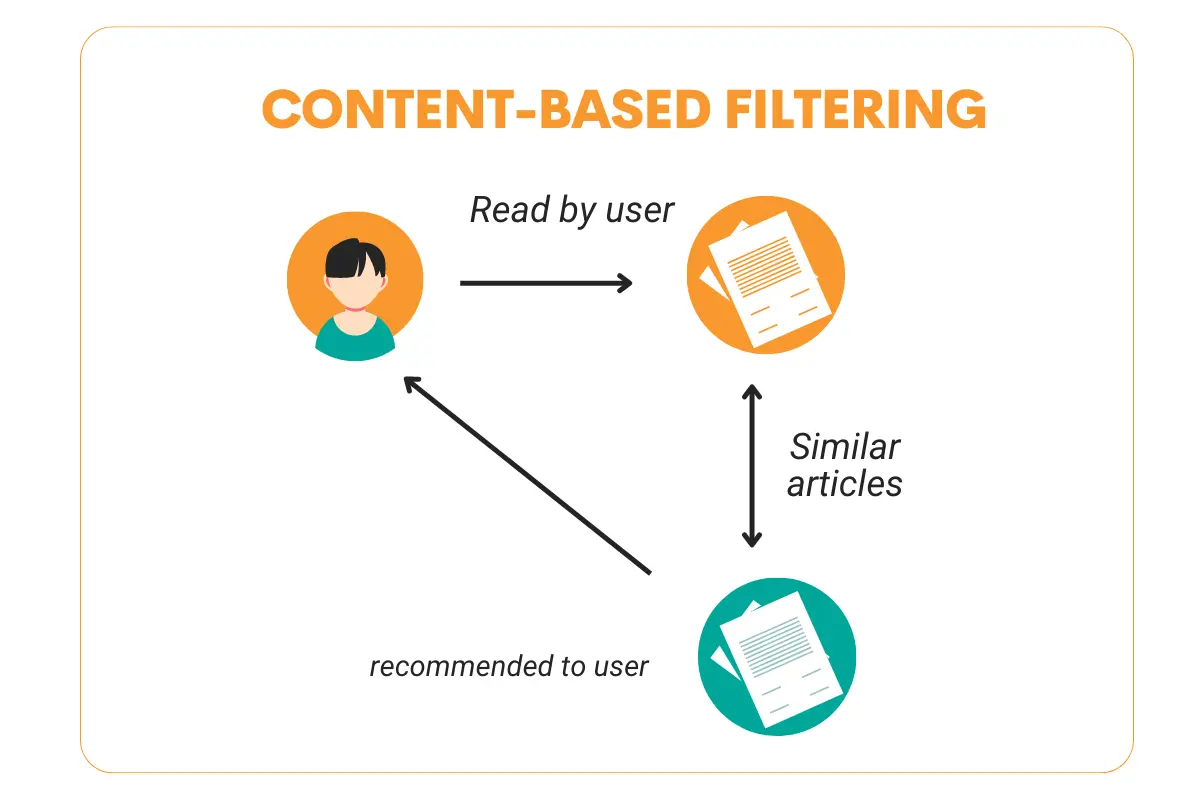
\includegraphics[width=0.6\linewidth]{image/content_base.png}
        \end{center}
        \caption[Poem]{ตัวอย่าง Content Based Filtering\cite{content_based}}
        \label{fig:content_based}
        \end{figure}
    \item Collaborative Filtering เป็นอีกเทคนิคหนึ่งในการแนะนำเนื้อหาให้กับผู้ใช้ วิธีการเบื้องต้นคือ ระบบจะแนะนำสิ่งที่น่าสนใจที่มาจากผู้ใช้อื่นที่มีข้อมูลเหมือนหรือคล้ายกัน เช่น เพศ, อายุ, เงินเดือน เป็นต้น 
    \begin{figure}[h] %h = here. other are top,bottom,separate page(p)
        \begin{center}
        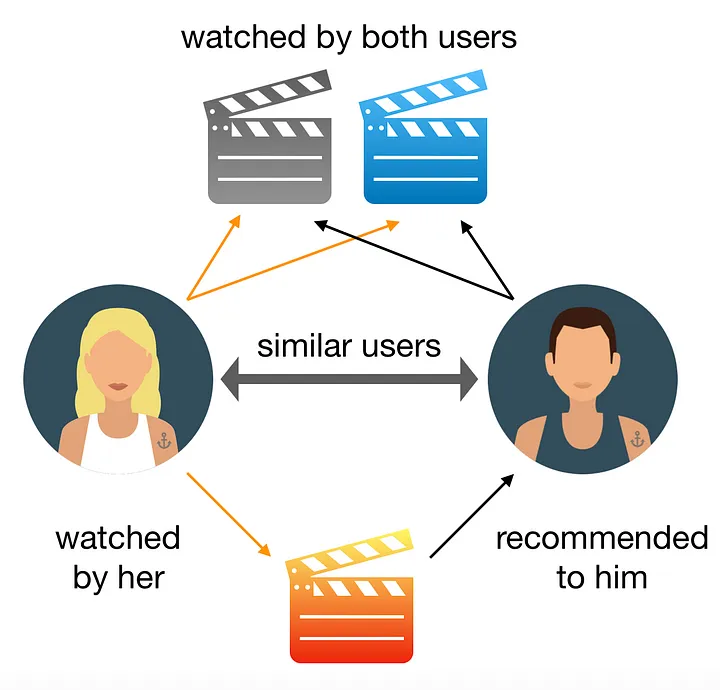
\includegraphics[width=0.6\linewidth]{image/collaborative.png}
        \end{center}
        \caption[Poem]{ตัวอย่าง Collaborative Filtering\cite{collaborative}}
        \label{fig:collaborative_filtering}
        \end{figure}
\end{enumerate}
\FloatBarrier

\subsection{K-nearest Neighbors}
K-Nearest Neighbors (K-NN) เป็นวิธีการแบ่งคลาสสำหรับใช้จัดหมวดหมู่ข้อมูล (Classification)ใช้หลักการเปรียบเทียบข้อมูลที่สนใจกับข้อมูลอื่นว่ามีความคล้ายคลึงมากน้อยเพียงใด หากข้อมูลที่กำลังสนใจนั้นอยู่ใกล้ข้อมูลใดมากที่สุด ระบบจะให้คำตอบเป็นเหมือนคำตอบของข้อมูลที่อยู่ใกล้ที่สุดนั้นลักษณะการทำงานแบบไม่ได้ใช้ข้อมูลชุดเรียนรู้ (training data) ในการสร้างแบบจำลองแต่จะใช้ข้อมูลนี้มาเป็นตัวแบบจำลองเลย
\cite{KNN}
\begin{figure}[h] %h = here. other are top,bottom,separate page(p)
    \begin{center}
        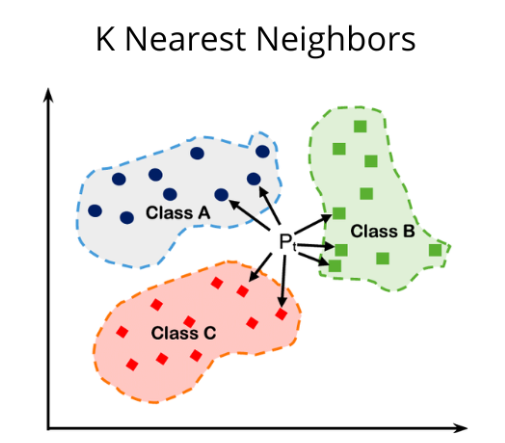
\includegraphics[width=0.4\linewidth]{image/knn.png}
    \end{center}
    \caption[Poem]{ตัวอย่าง K Nearest Neighbors}
    \label{fig:knn}
\end{figure}





% \subsection{Subsection heading goes here}

% Subsection 1 text

% \subsubsection{Subsubsection 1 heading goes here}
% Subsubsection 1 text

% \subsubsection{Subsubsection 2 heading goes here}
% Subsubsection 2 text

% \section{Third section}
% Section 3 text. The dielectric constant\index{dielectric constant}
% at the air-metal interface determines
% the resonance shift\index{resonance shift} as absorption or capture occurs
% is shown in Equation~\eqref{eq:dielectric}:

% \begin{equation}\label{eq:dielectric}
% k_1=\frac{\omega}{c({1/\varepsilon_m + 1/\varepsilon_i})^{1/2}}=k_2=\frac{\omega
% \sin(\theta)\varepsilon_\mathit{air}^{1/2}}{c}
% \end{equation}

% \noindent
% where $\omega$ is the frequency of the plasmon, $c$ is the speed of
% light, $\varepsilon_m$ is the dielectric constant of the metal,
% $\varepsilon_i$ is the dielectric constant of neighboring insulator,
% and $\varepsilon_\mathit{air}$ is the dielectric constant of air.

% \section{About using figures in your report}

% % define a command that produces some filler text, the lorem ipsum.
% \newcommand{\loremipsum}{
%   \textit{Lorem ipsum dolor sit amet, consectetur adipisicing elit, sed do
%   eiusmod tempor incididunt ut labore et dolore magna aliqua. Ut enim ad
%   minim veniam, quis nostrud exercitation ullamco laboris nisi ut
%   aliquip ex ea commodo consequat. Duis aute irure dolor in
%   reprehenderit in voluptate velit esse cillum dolore eu fugiat nulla
%   pariatur. Excepteur sint occaecat cupidatat non proident, sunt in
%   culpa qui officia deserunt mollit anim id est laborum.}\par}

% \begin{figure}
%   \centering

%   \fbox{
%      \parbox{.6\textwidth}{\loremipsum}
%   }

%   % To include an image in the figure, say myimage.pdf, you could use
%   % the following code. Look up the documentation for the package
%   % graphicx for more information.
%   % \includegraphics[width=\textwidth]{myimage}

%   \caption[Sample figure]{This figure is a sample containing \gls{lorem ipsum},
%   showing you how you can include figures and glossary in your report.
%   You can specify a shorter caption that will appear in the List of Figures.}
%   \label{fig:sample-figure}
% \end{figure}

% Using \verb.\label. and \verb.\ref. commands allows us to refer to
% figures easily. If we can refer to Figures
% \ref{fig:walrus} and \ref{fig:sample-figure} by name in the {\LaTeX}
% source code, then we will not need to update the code that refers to it
% even if the placement or ordering of the figures changes.

% \loremipsum\loremipsum

% % This code demonstrates how to get a landscape table or figure. It
% % uses the package lscape to turn everything but the page number into
% % landscape orientation. Everything should be included within an
% % \afterpage{ .... } to avoid causing a page break too early.
% \afterpage{
%   \begin{landscape}
%   \begin{table}
%     \caption{Sample landscape table}
%     \label{tab:sample-table}

%     \centering

%     \begin{tabular}{c||c|c}
%         Year & A & B \\
%         \hline\hline
%         1989 & 12 & 23 \\
%         1990 & 4 & 9 \\
%         1991 & 3 & 6 \\
%     \end{tabular}
%   \end{table}
%   \end{landscape}
% }

% \loremipsum\loremipsum\loremipsum

% \section{Overfull hbox}

% When the \verb.semifinal. option is passed to the \verb.cpecmu. document class,
% any line that is longer than the line width, i.e., an overfull hbox, will be
% highlighted with a black solid rule:
% \begin{center}
% \begin{minipage}{2em}
% juxtaposition
% \end{minipage}
% \end{center}

\section{\ifenglish%
\ifcpe CPE \else ISNE \fi knowledge used, applied, or integrated in this project
\else%
ความรู้ตามหลักสูตรซึ่งถูกนำมาใช้หรือบูรณาการในโครงงาน
\fi
}
\begin{enumerate}
    \item ความรู้ด้าน Human Computer Interaction ใช้ในการออกแบบดีไซน์หน้าเว็บให้สื่อประสานกับกลุ่มผู้ใช้งานเป้าหมาย (269492)
    \item ความรู้ด้าน Natural Language Processing ใช้ประยุกต์ในการพัฒนาระบบแนะนำกิจกรรม (261499)
    \item ความรู้ด้าน Web Development ใช้ในการพัฒนาเว็บไซต์ (261207)
    \item ความรู้ด้าน Database ใช้ในการออกแบบฐานข้อมูล (261342)
    \item ความรู้ด้าน Infra and Cloud technology ใช้ในการdeployหน้าเว็บ (261494)
\end{enumerate}


\section{\ifenglish%
Extracurricular knowledge used, applied, or integrated in this project
\else%
ความรู้นอกหลักสูตรซึ่งถูกนำมาใช้หรือบูรณาการในโครงงาน
\fi
}
\begin{enumerate}
    \item ความรู้เรื่องการใช้ MongoDB ในการสร้างฐานข้อมูล
    \item ความรู้ด้าน Data Visualization มาใช้ในการสร้างหน้า Dashboard
    \item ความรู้ด้าน Data Science ในการนำข้อมูลมาวิเคราะห์
\end{enumerate}


\chapter{\ifproject%
\ifenglish Project Structure and Methodology\else โครงสร้างและขั้นตอนการทำงาน\fi
\else%
\ifenglish Project Structure\else โครงสร้างของโครงงาน\fi
\fi
}

% ในบทนี้จะกล่าวถึงหลักการ และการออกแบบระบบ

\makeatletter

% \renewcommand\section{\@startsection {section}{1}{\z@}%
%                                    {13.5ex \@plus -1ex \@minus -.2ex}%
%                                    {2.3ex \@plus.2ex}%
%                                    {\normalfont\large\bfseries}}

\makeatother
%\vspace{2ex}
% \titleformat{\section}{\normalfont\bfseries}{\thesection}{1em}{}
% \titlespacing*{\section}{0pt}{10ex}{0pt}



\section{หลักการทำงานของแอปพลิเคชัน}
โครงงานนี้เป็นแอปพลิเคชันที่ช่วยในการสร้าง, ประกาศกิจกรรม และเข้าร่วมกิจกรรมของนักศึกษาและบุคลากรของมหาวิทยาลัยเชียงใหม่ที่มี CMU-Account
โดยเลือกพัฒนาเป็นเว็บแอปพลิเคชัน มีระบบที่ให้ผู้ใช้สร้างและประชาสัมพันธ์กิจกรรม, ดูข้อมูลและขอเข้าร่วมกิจกรรมที่ตนเองสนใจ โดยทางเว็บจะมีระบบแนะนำกิจกรรมที่ตรงกับความสนใจของผู้ใช้มากที่สุด และยังมีการนำสถิติการใช้งานเว็บแอปพลิเคชันในส่วนต่างๆมาวิเคราะห์และนำเสนอในรูปแบบที่เข้าใจง่าย โดยใช้ความรู้ด้าน Data Visualization
\begin{figure}[h] %h = here. other are top,bottom,separate page(p)
\begin{center}
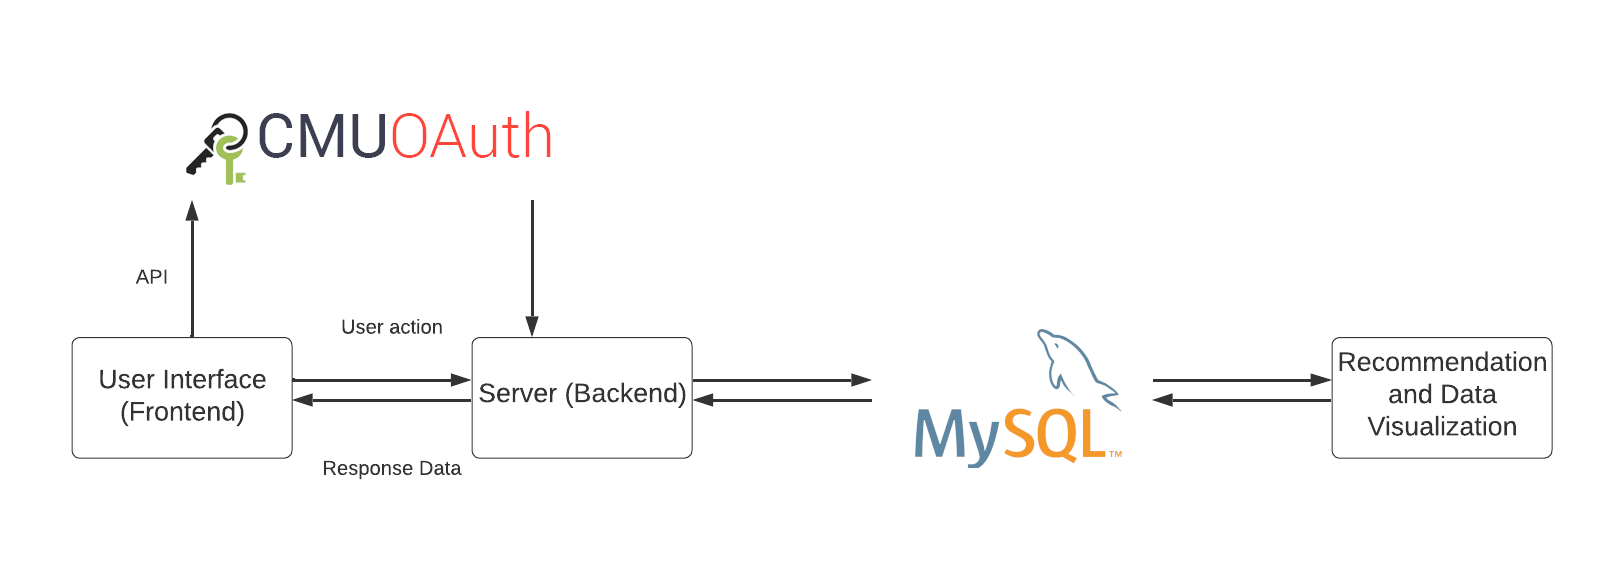
\includegraphics[width=0.9\linewidth]{image/31_system_overview.png}
\end{center}
\caption[Poem]{System Overview}
\label{fig:system_overview}
\end{figure}
\section{การใช้งานแอปพลิเคชัน}
เว็บแอปพลิเคชันนี้จะแบ่งกลุ่มผู้ใช้ออกเป็น 2 กลุ่ม ได้แก่
\subsection{ผู้ใช้ทั่วไป}
สิ่งที่ผู้ใช้ทั่วไปสามารถใช้งานได้ ได้แก่
\begin{itemize}
    \item สามารถค้นหากิจกรรมได้ ทั้งจากการพิมพ์คำสำคัญ ในช่องค้นหา และหน้าข่าวสารกิจกรรมทั้งหมด
    \item สามารถดูรายละเอียดของแต่ละกิจกรรมได้
    \item อ่านความคิดเห็นของแต่ละกิจกรรมได้
    \item ติดต่อสอบถาม หรือส่งข้อเสนอแนะเกี่ยวกับเว็บแอปพลิเคชันได้
\end{itemize}
\subsection{ผู้ใช้ที่ยืนยันตัวตนด้วย CMU-OAuth}
หลังจากผู้ใช้ลงทะเบียนเข้าใช้งานด้วย CMU Account แล้ว สิ่งที่ผู้ใช้สามารถทำได้เพิ่มมากขึ้น ได้แก่
\begin{itemize}
    \item สามารถตั้งชื่อ username เพื่อใช้เป็นนามแฝงได้
    \item สร้างกิจกรรมใหม่ขึ้นมา ทั้งแบบต้องการสมาชิกหรือแค่ประชาสัมพันธ์กิจกรรม
    \item แสดงความคิดเห็นในแต่ละหน้ากิจกรรมได้
    \item สามารถสมัครเข้าร่วมกิจกรรมที่สนใจได้
    \item สามารถดูปฏิทินเพื่อตรวจสอบวัน/เวลาแต่ละกิจกรรมได้
    \item สามารถเข้าหน้า Dashboard เพื่อดูข้อมูลสถิติของเว็บได้
\end{itemize}
\section{นโยบายความเป็นส่วนตัว}
เมื่อผู้ใช้ลงชื่อเข้าใช้งานครั้งแรก ผู้ใช้จะต้องตั้งค่า username เพื่อใช้เป็นนามแฝงในการแสดงความคิดเห็นในหน้ากิจกรรม

\section{การออกแบบหน้าเว็บแอปพลิเคชัน}
ในการออกแบบหน้าเว็บแอปพลิชัน พวกเราได้เลือกใช้ Figma เพราะเป็นเครื่องมือที่อำนวยความสะดวก ในการออกแบบหน้าเว็บแอปพลิเคชัน ช่วยให้การออกแบบ UI/UX สะดวกมากขึ้น อีกทั้งยังเป็นเครื่องมือที่ผู้คนต่างก็นิยมใช้
ทำให้ผู้ใช้ทั่วโลกสามารถแชร์วิธีการออกแบบ ทำให้สามารถนำไปเป็นไอเดียในการออกแบบได้ 
\begin{figure}[h]
\begin{center}

\includegraphics[width=0.5\linewidth]{image/Figma-design/Main-not-login.png}
\end{center}
\caption[Poem]{หน้าแรก}
\label{fig:main}
\end{figure}

\begin{figure}[h]
  \centering
  \begin{subfigure}[b]{0.3\linewidth}
    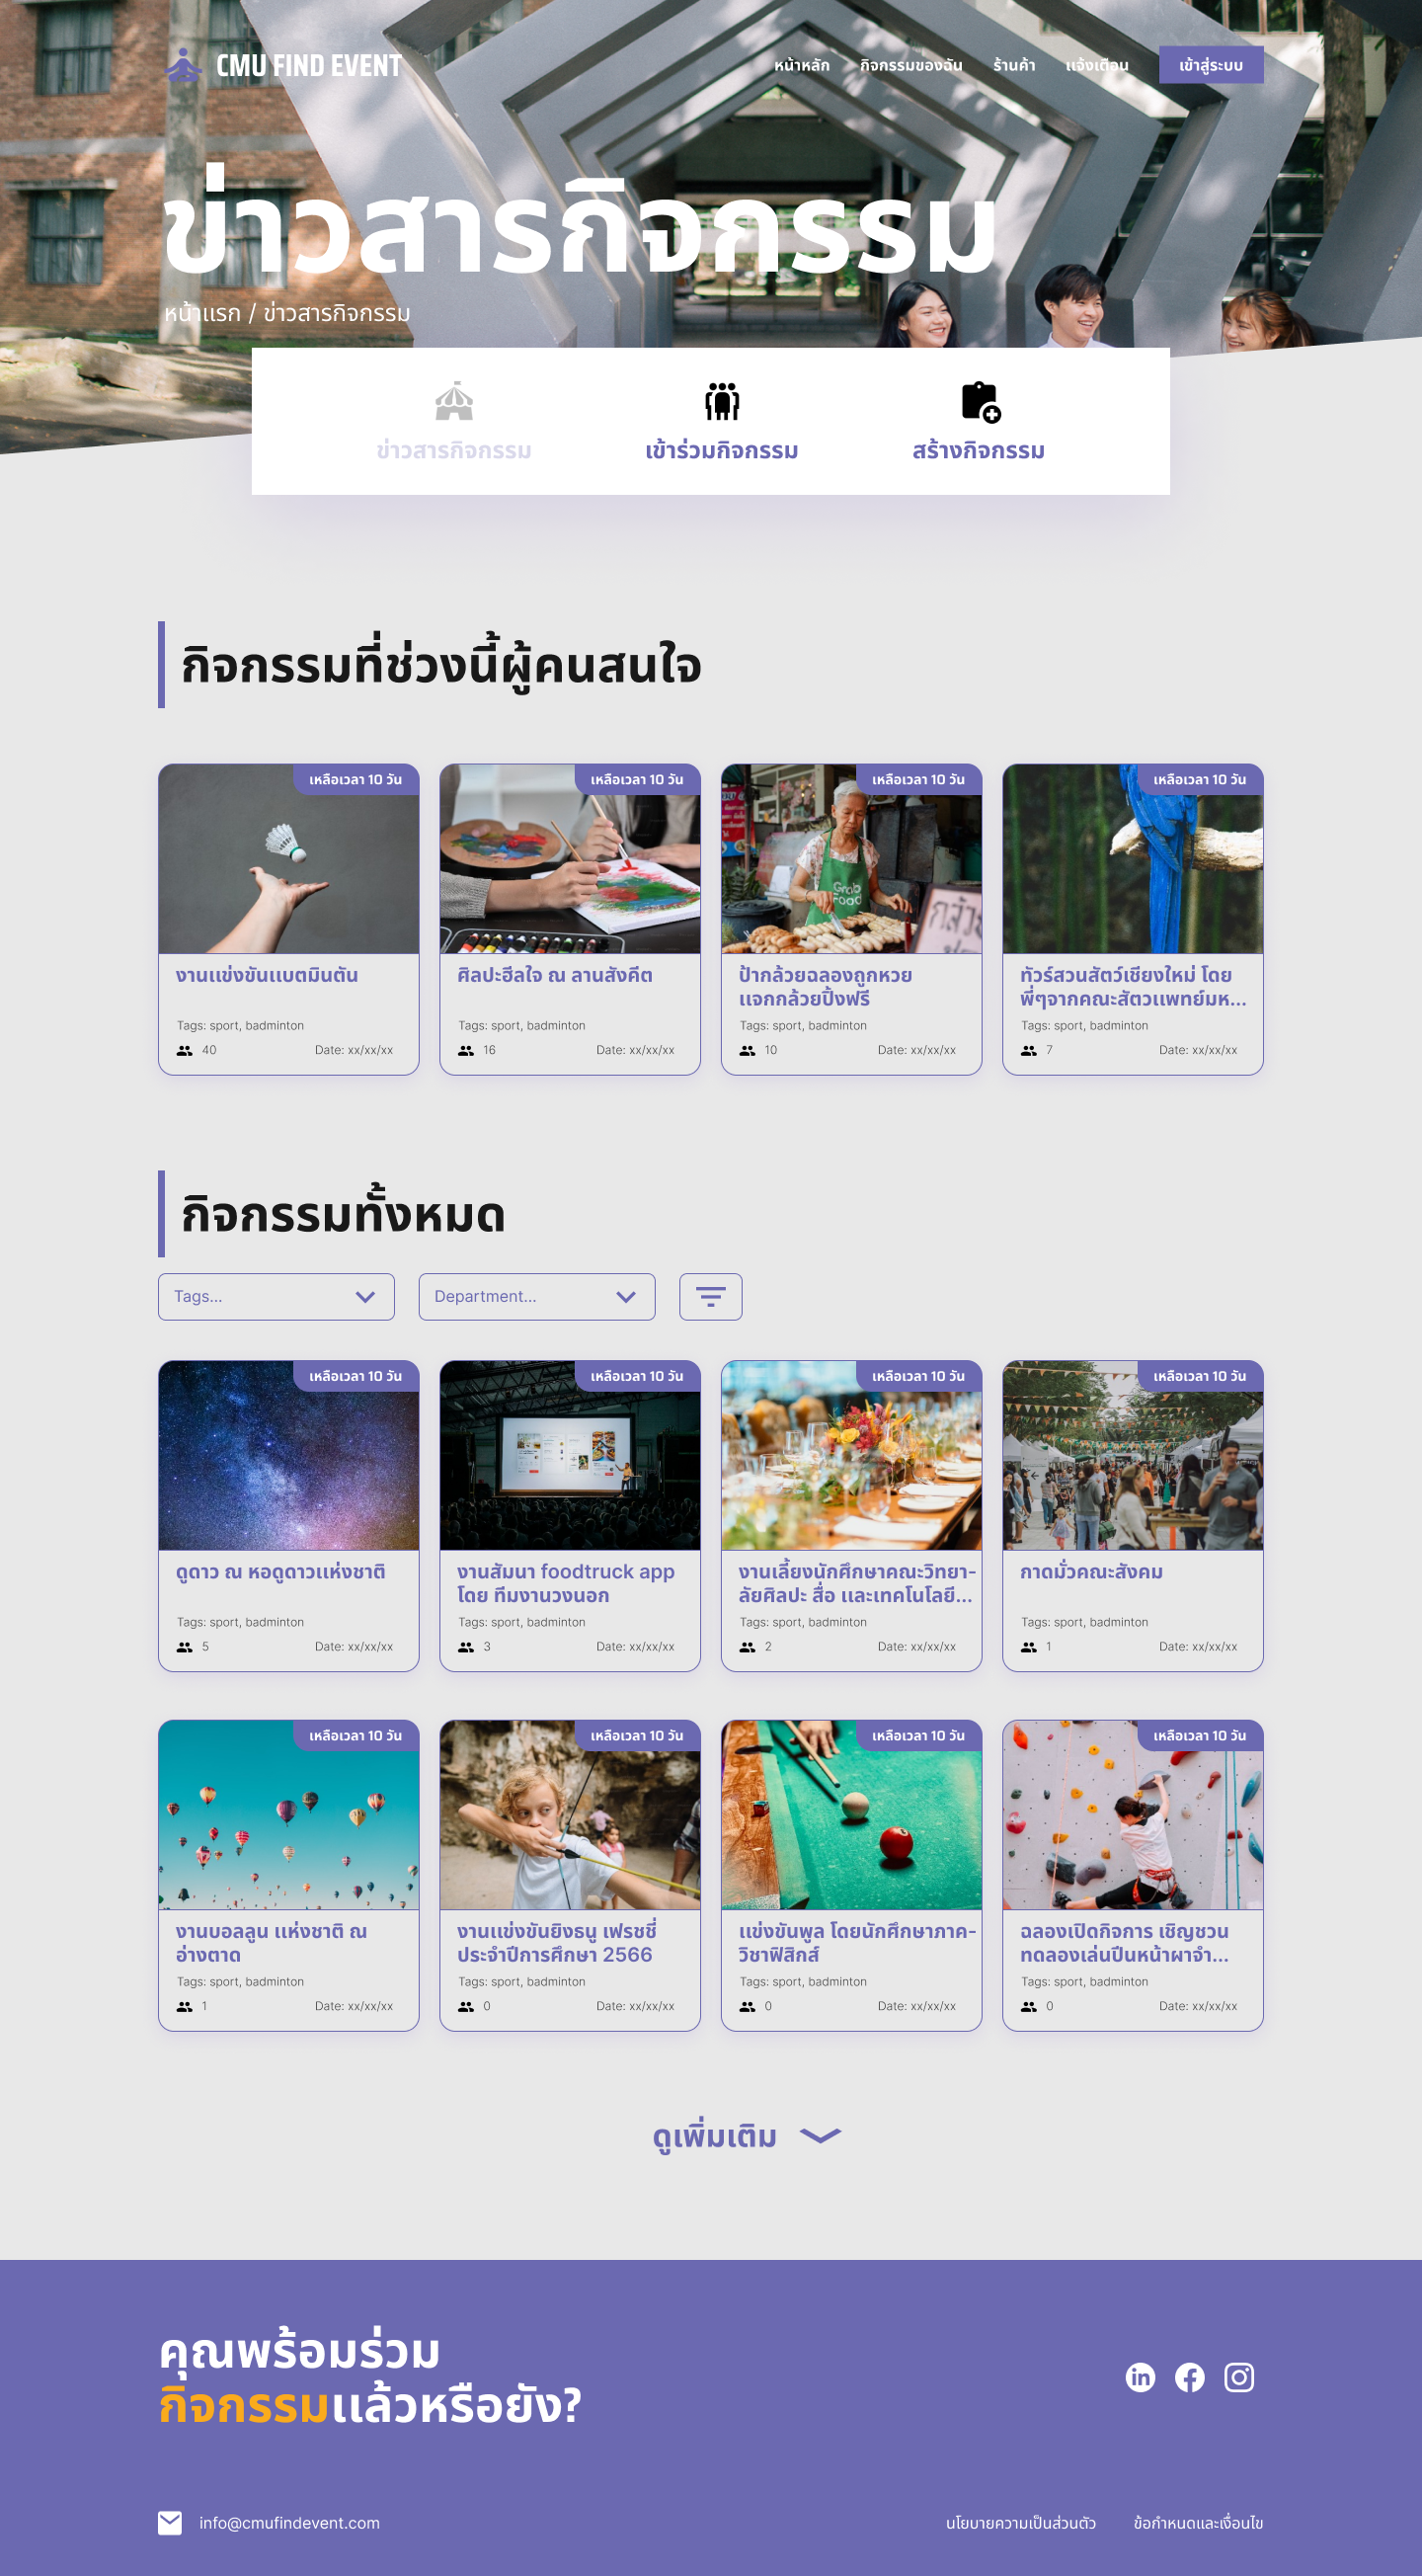
\includegraphics[width=\linewidth]{image/Figma-design/Event-info.png}
    \caption{แสดงรายการประกิจกรรม}
  \end{subfigure}
  \hfill
  \begin{subfigure}[b]{0.3\linewidth}
    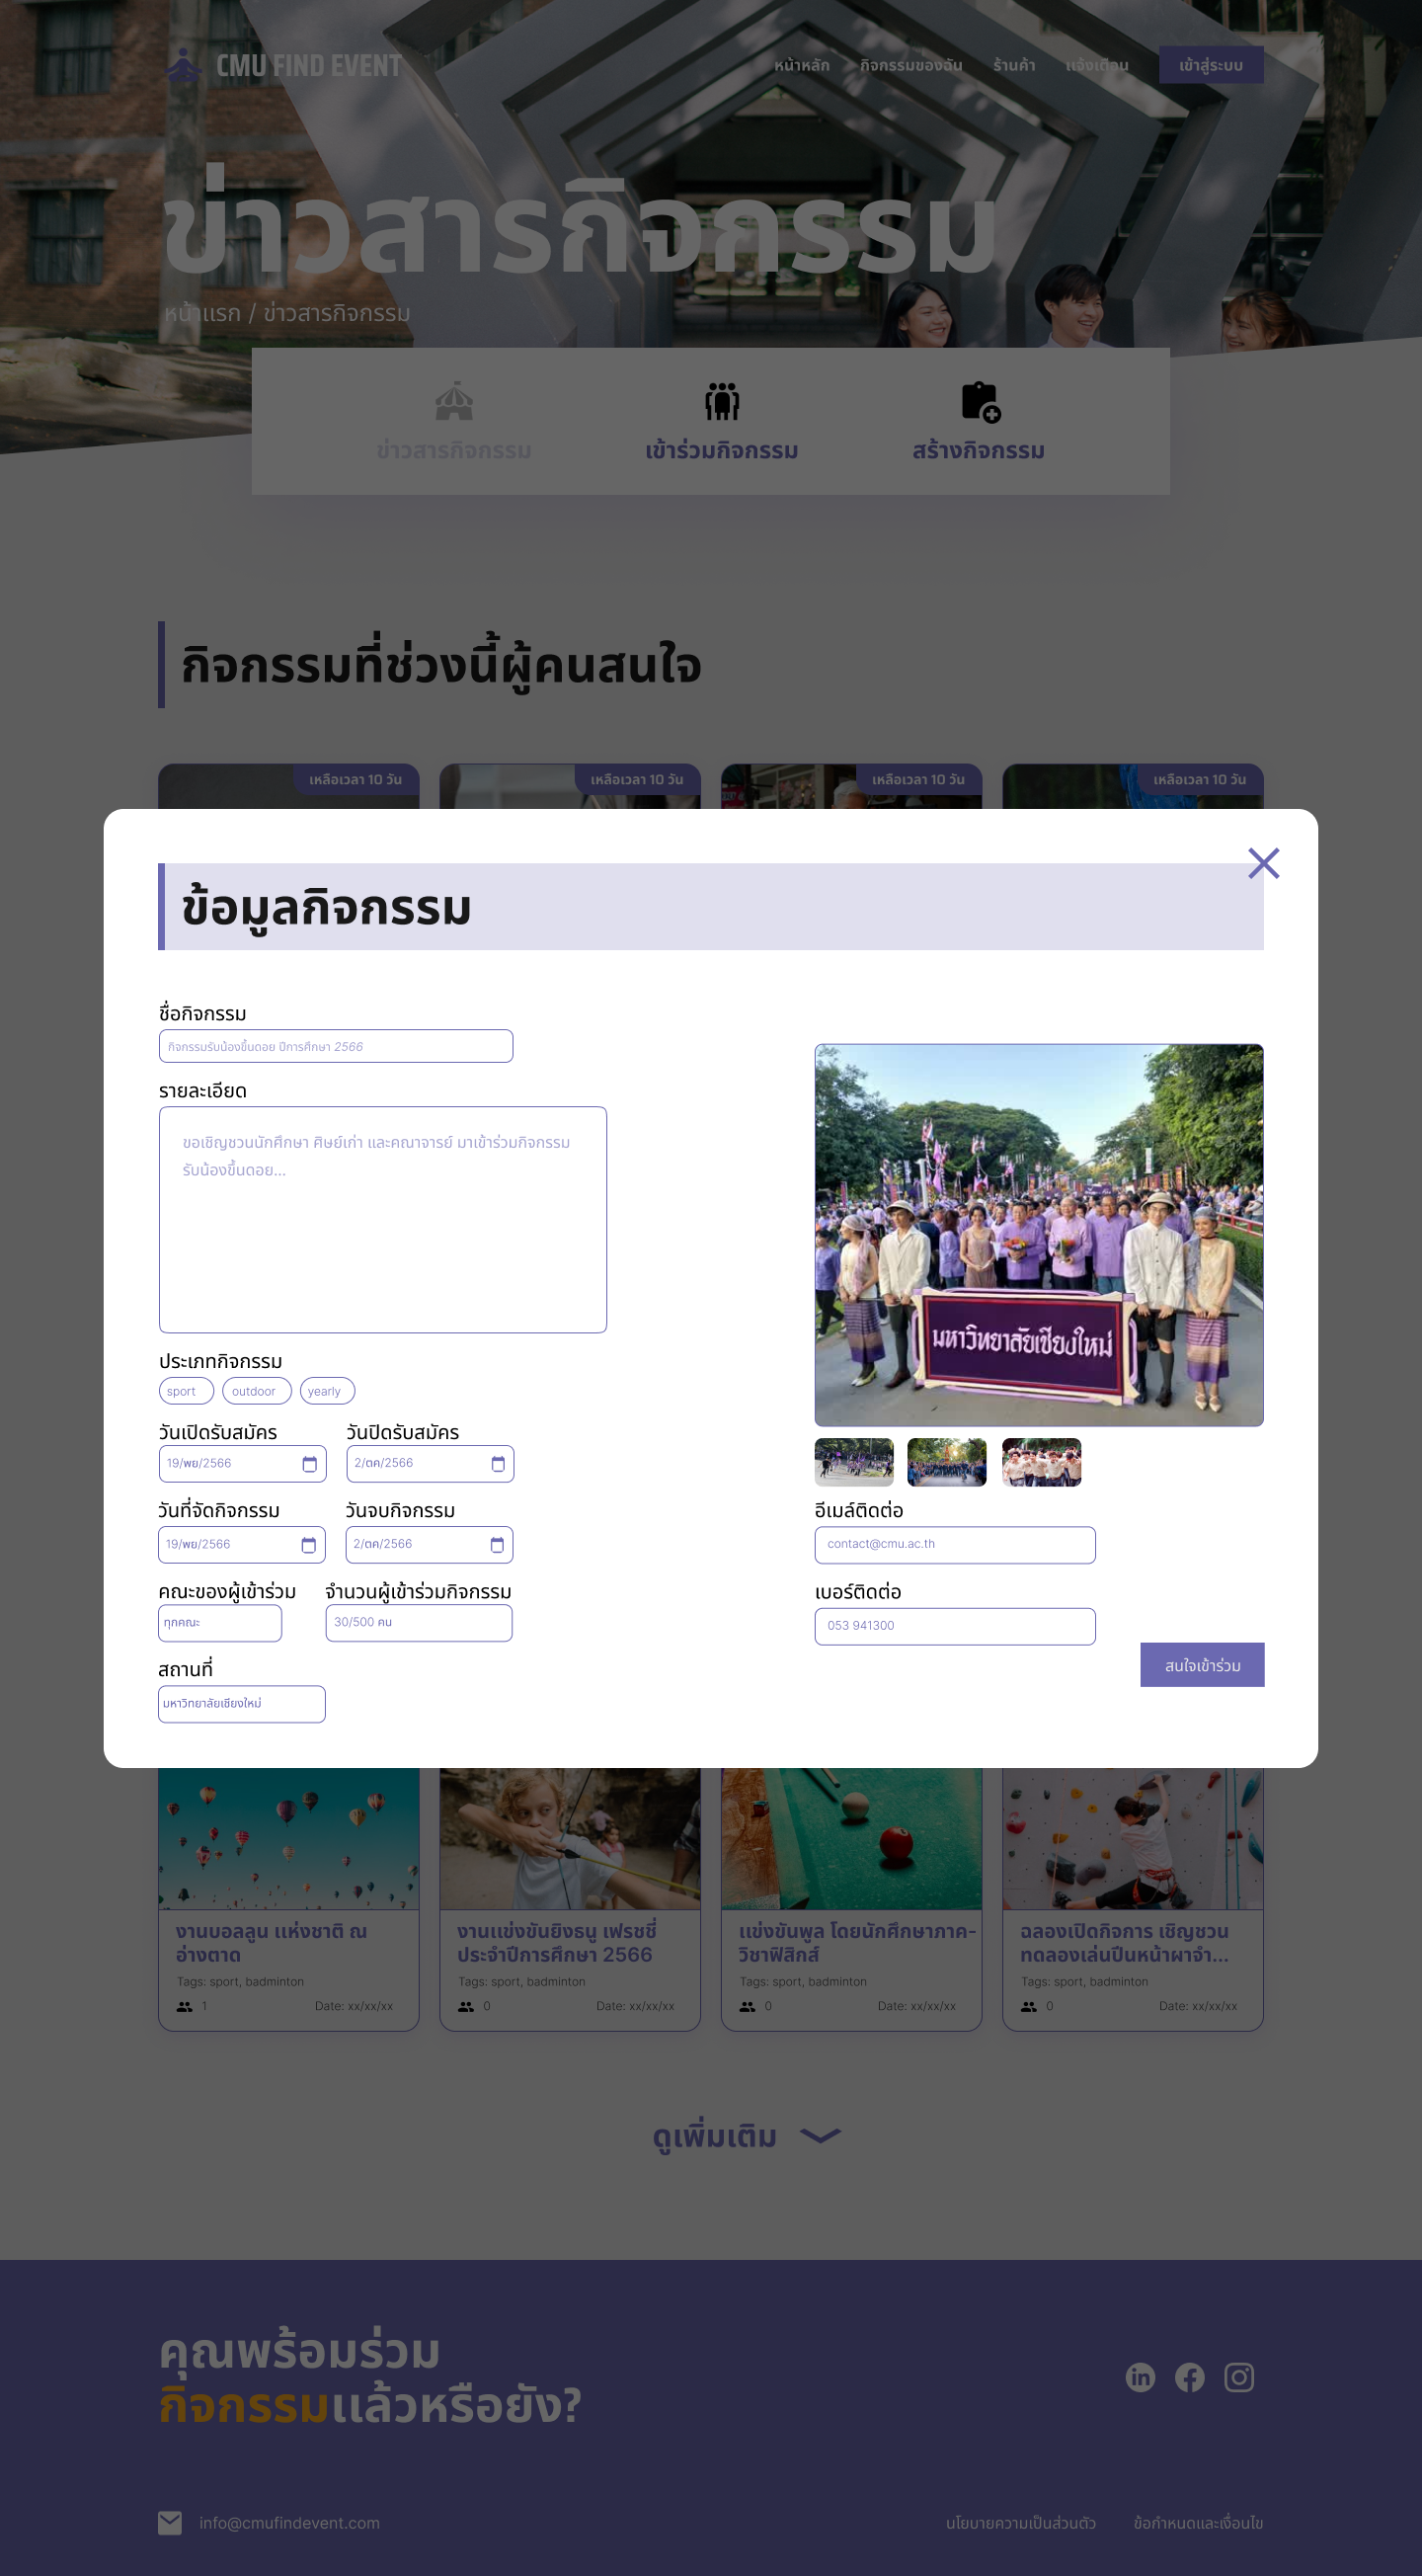
\includegraphics[width=\linewidth]{image/Figma-design/Event-info-1.png}
    \caption{แสดงรายละเอียดของประกาศกิจกรรม}
  \end{subfigure}
  \caption{หน้าข่าวสารกิจกรรม}
  \label{fig:event-info}
\end{figure}

\begin{figure}[h]
  \centering
  \begin{subfigure}[b]{0.3\linewidth}
    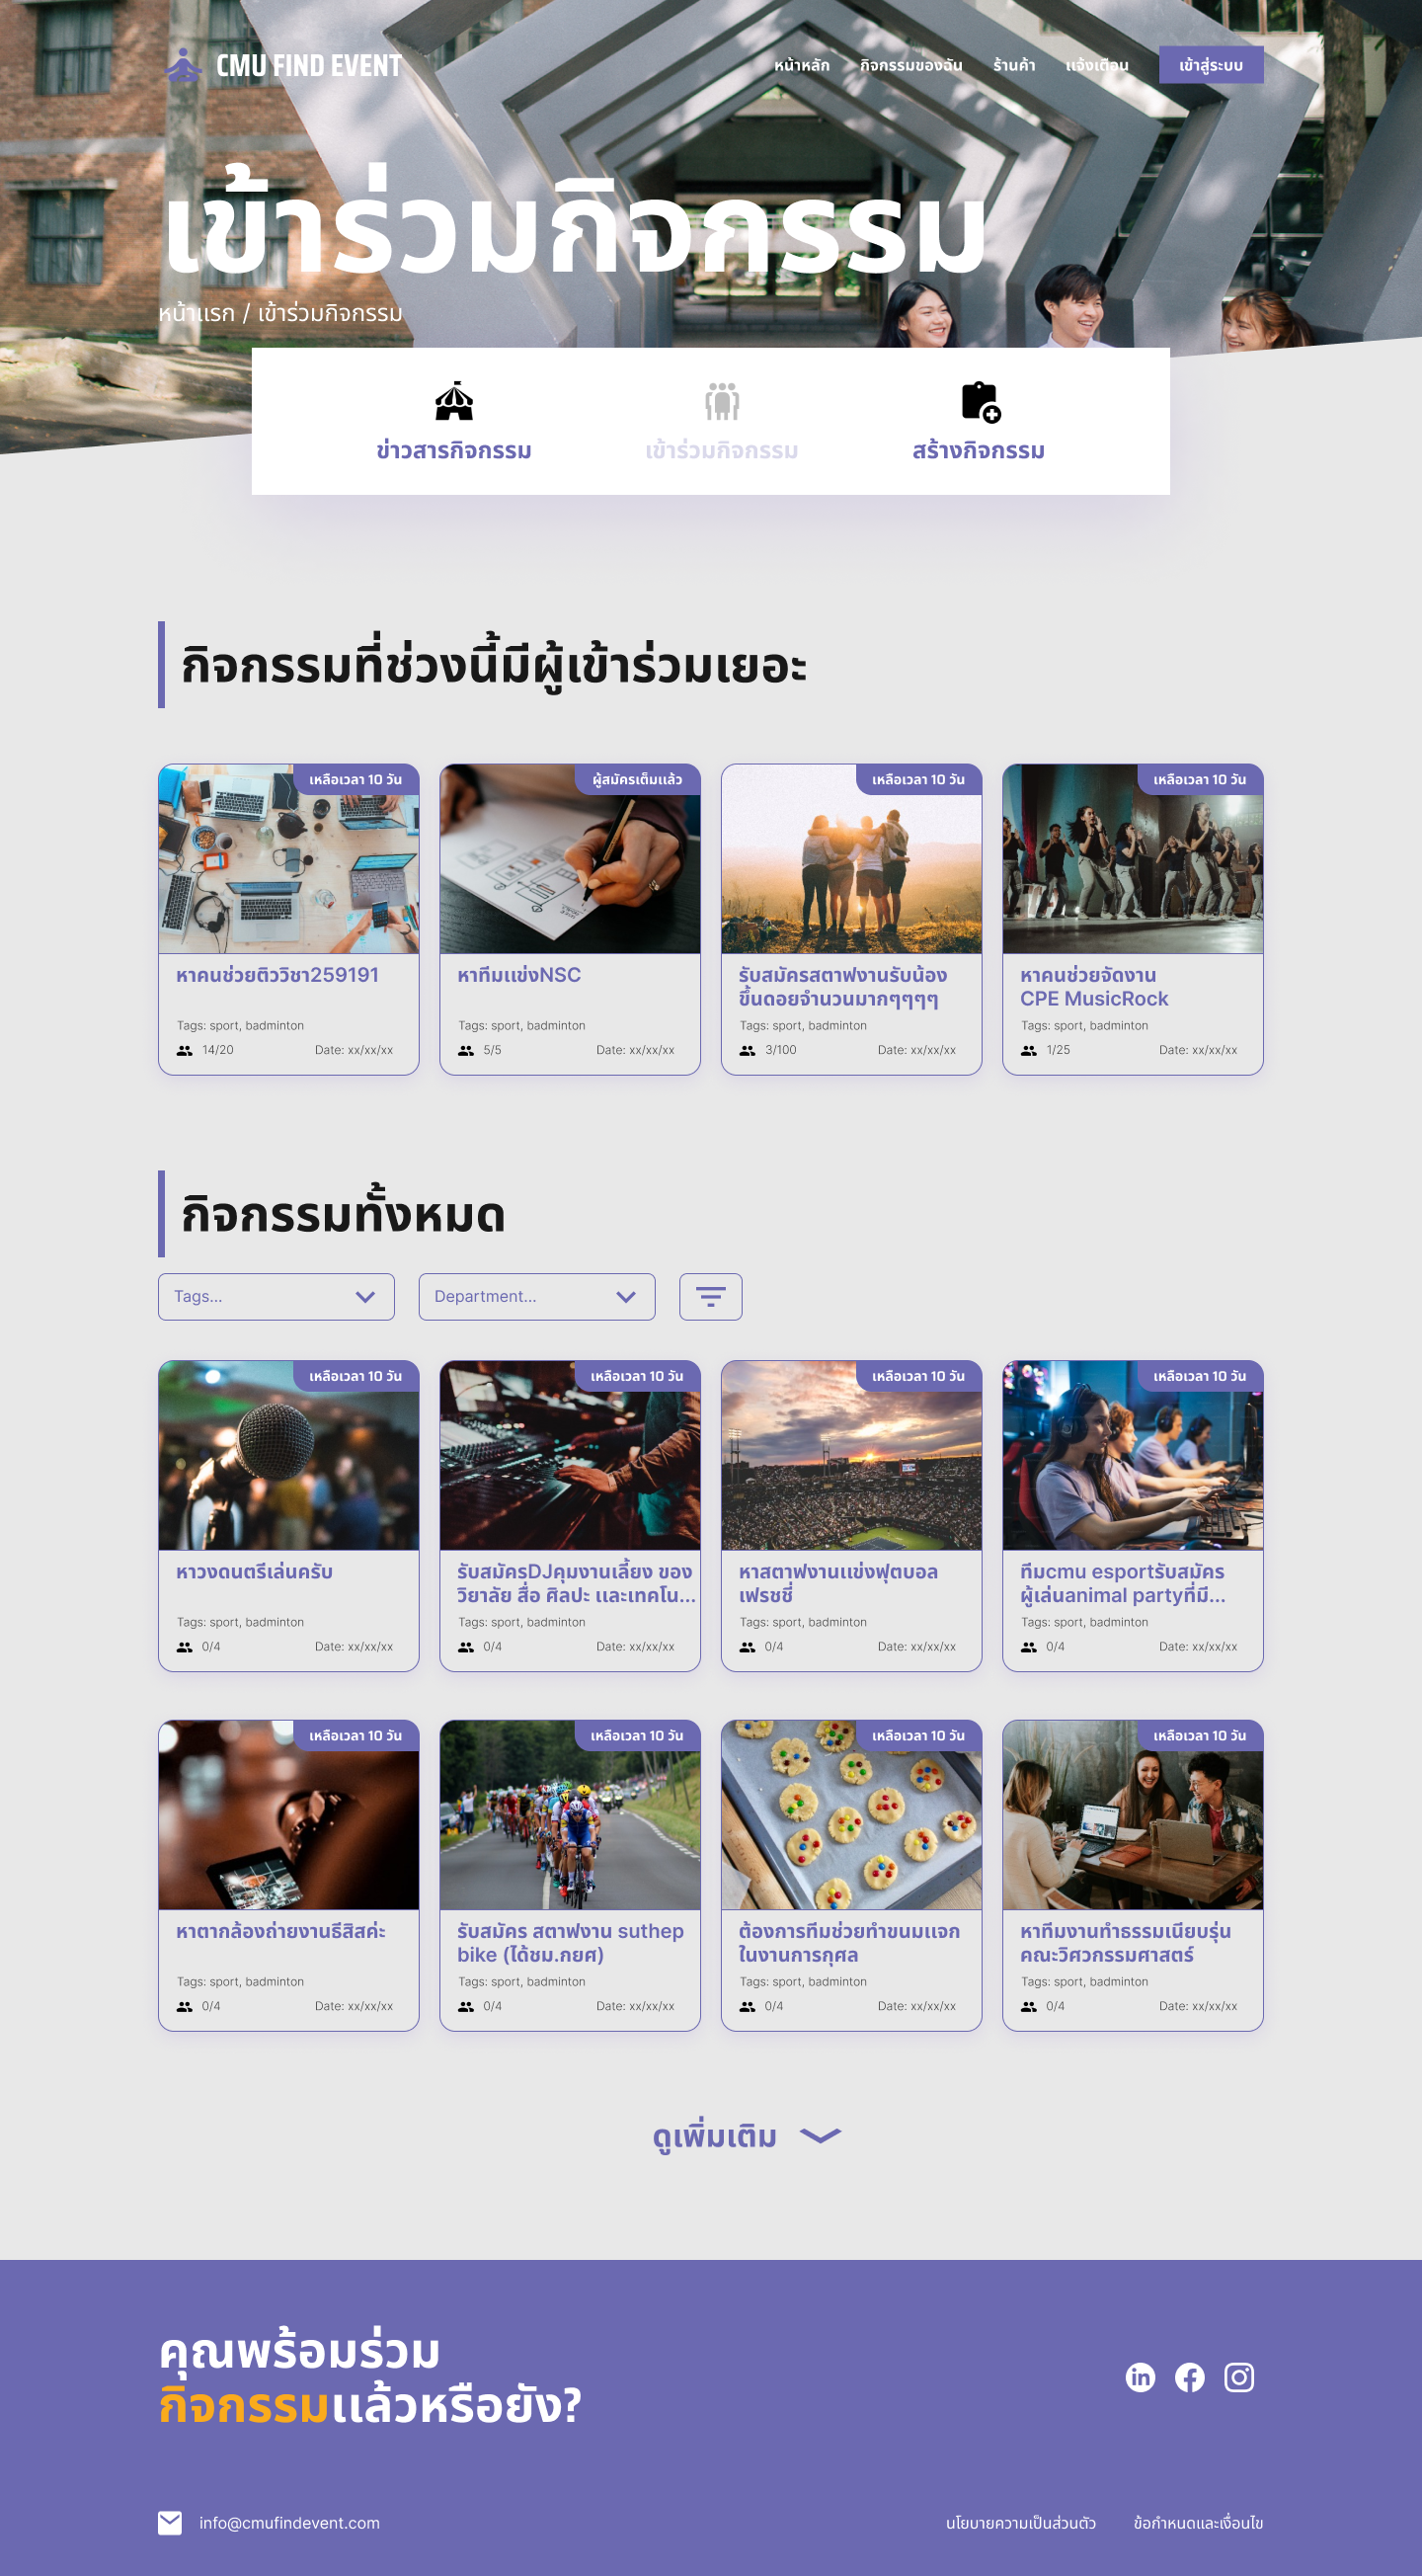
\includegraphics[width=\linewidth]{image/Figma-design/Event-join.png}
    \caption{แสดงรายการกิจกรรมที่เปิดรับสมัคร}
  \end{subfigure}
  \hfill
  \begin{subfigure}[b]{0.3\linewidth}
    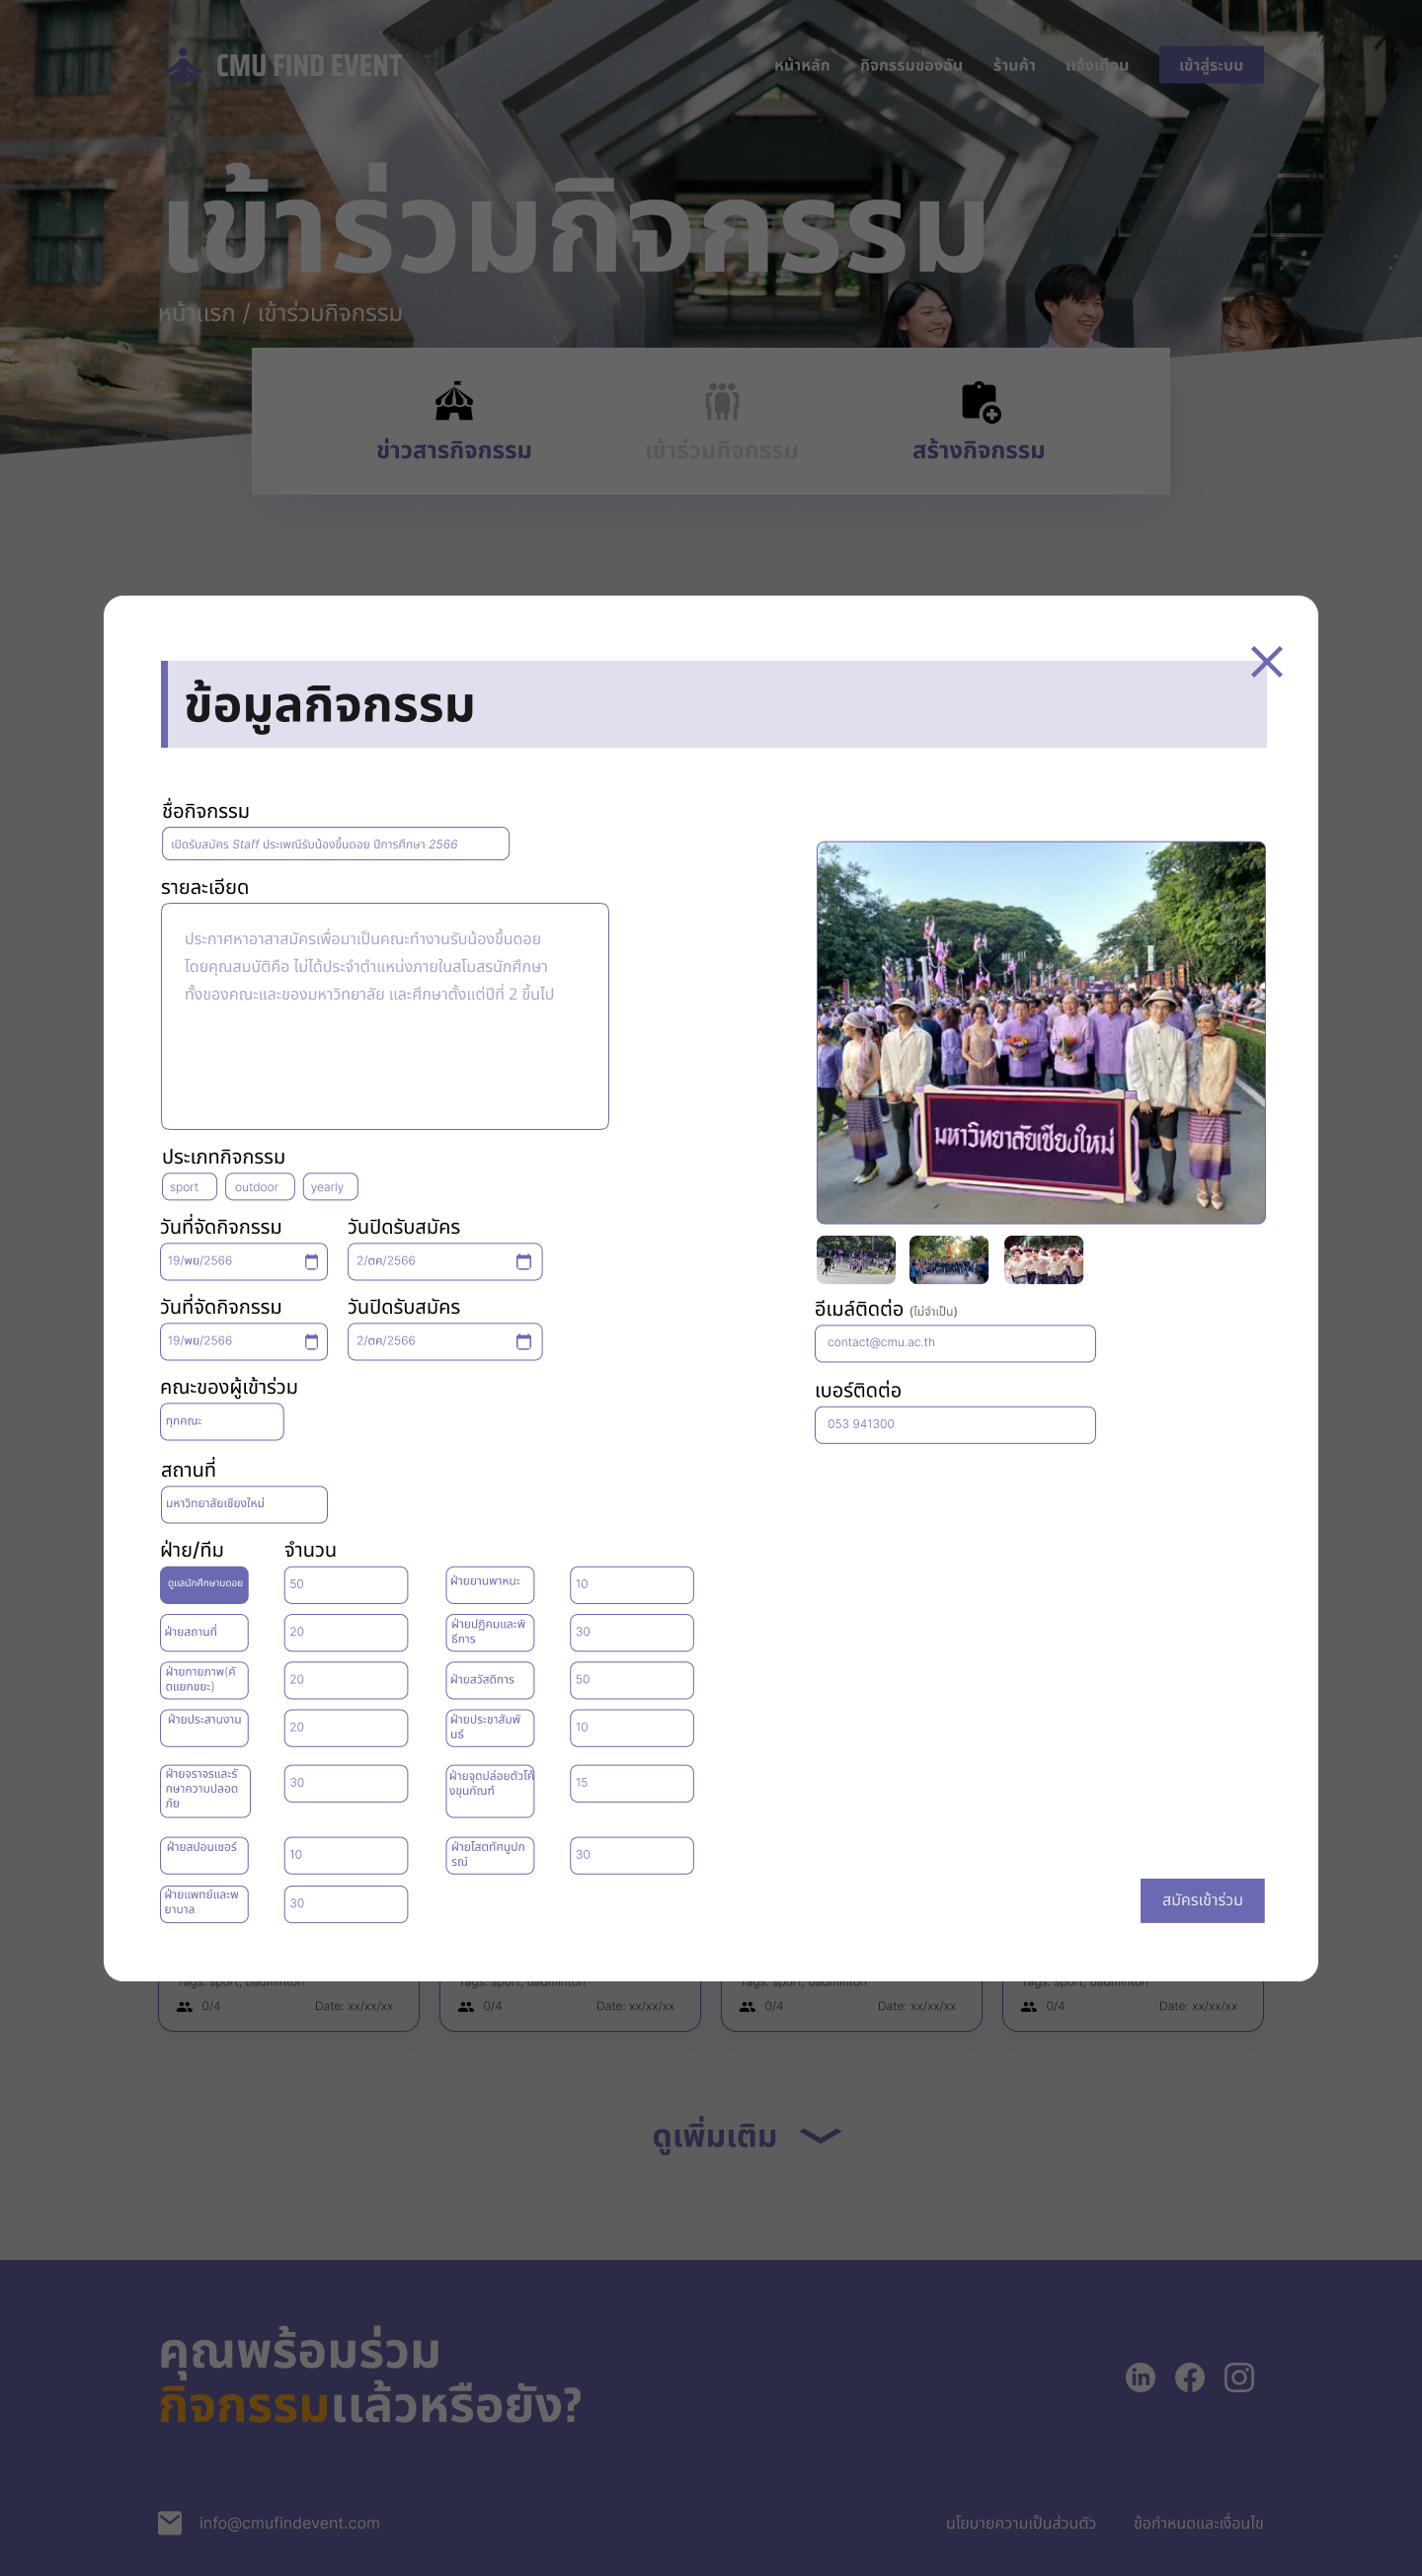
\includegraphics[width=\linewidth]{image/Figma-design/Event-join-1.png}
    \caption{แสดงรายละเอียดของกิจกรรมที่เปิดรับสมัคร}
  \end{subfigure}
  \caption{หน้าเข้าร่วมกิจกรรม}
  \label{fig:event-join}
\end{figure}

\begin{figure}[h]
  \centering
  \begin{subfigure}[b]{0.3\linewidth}
    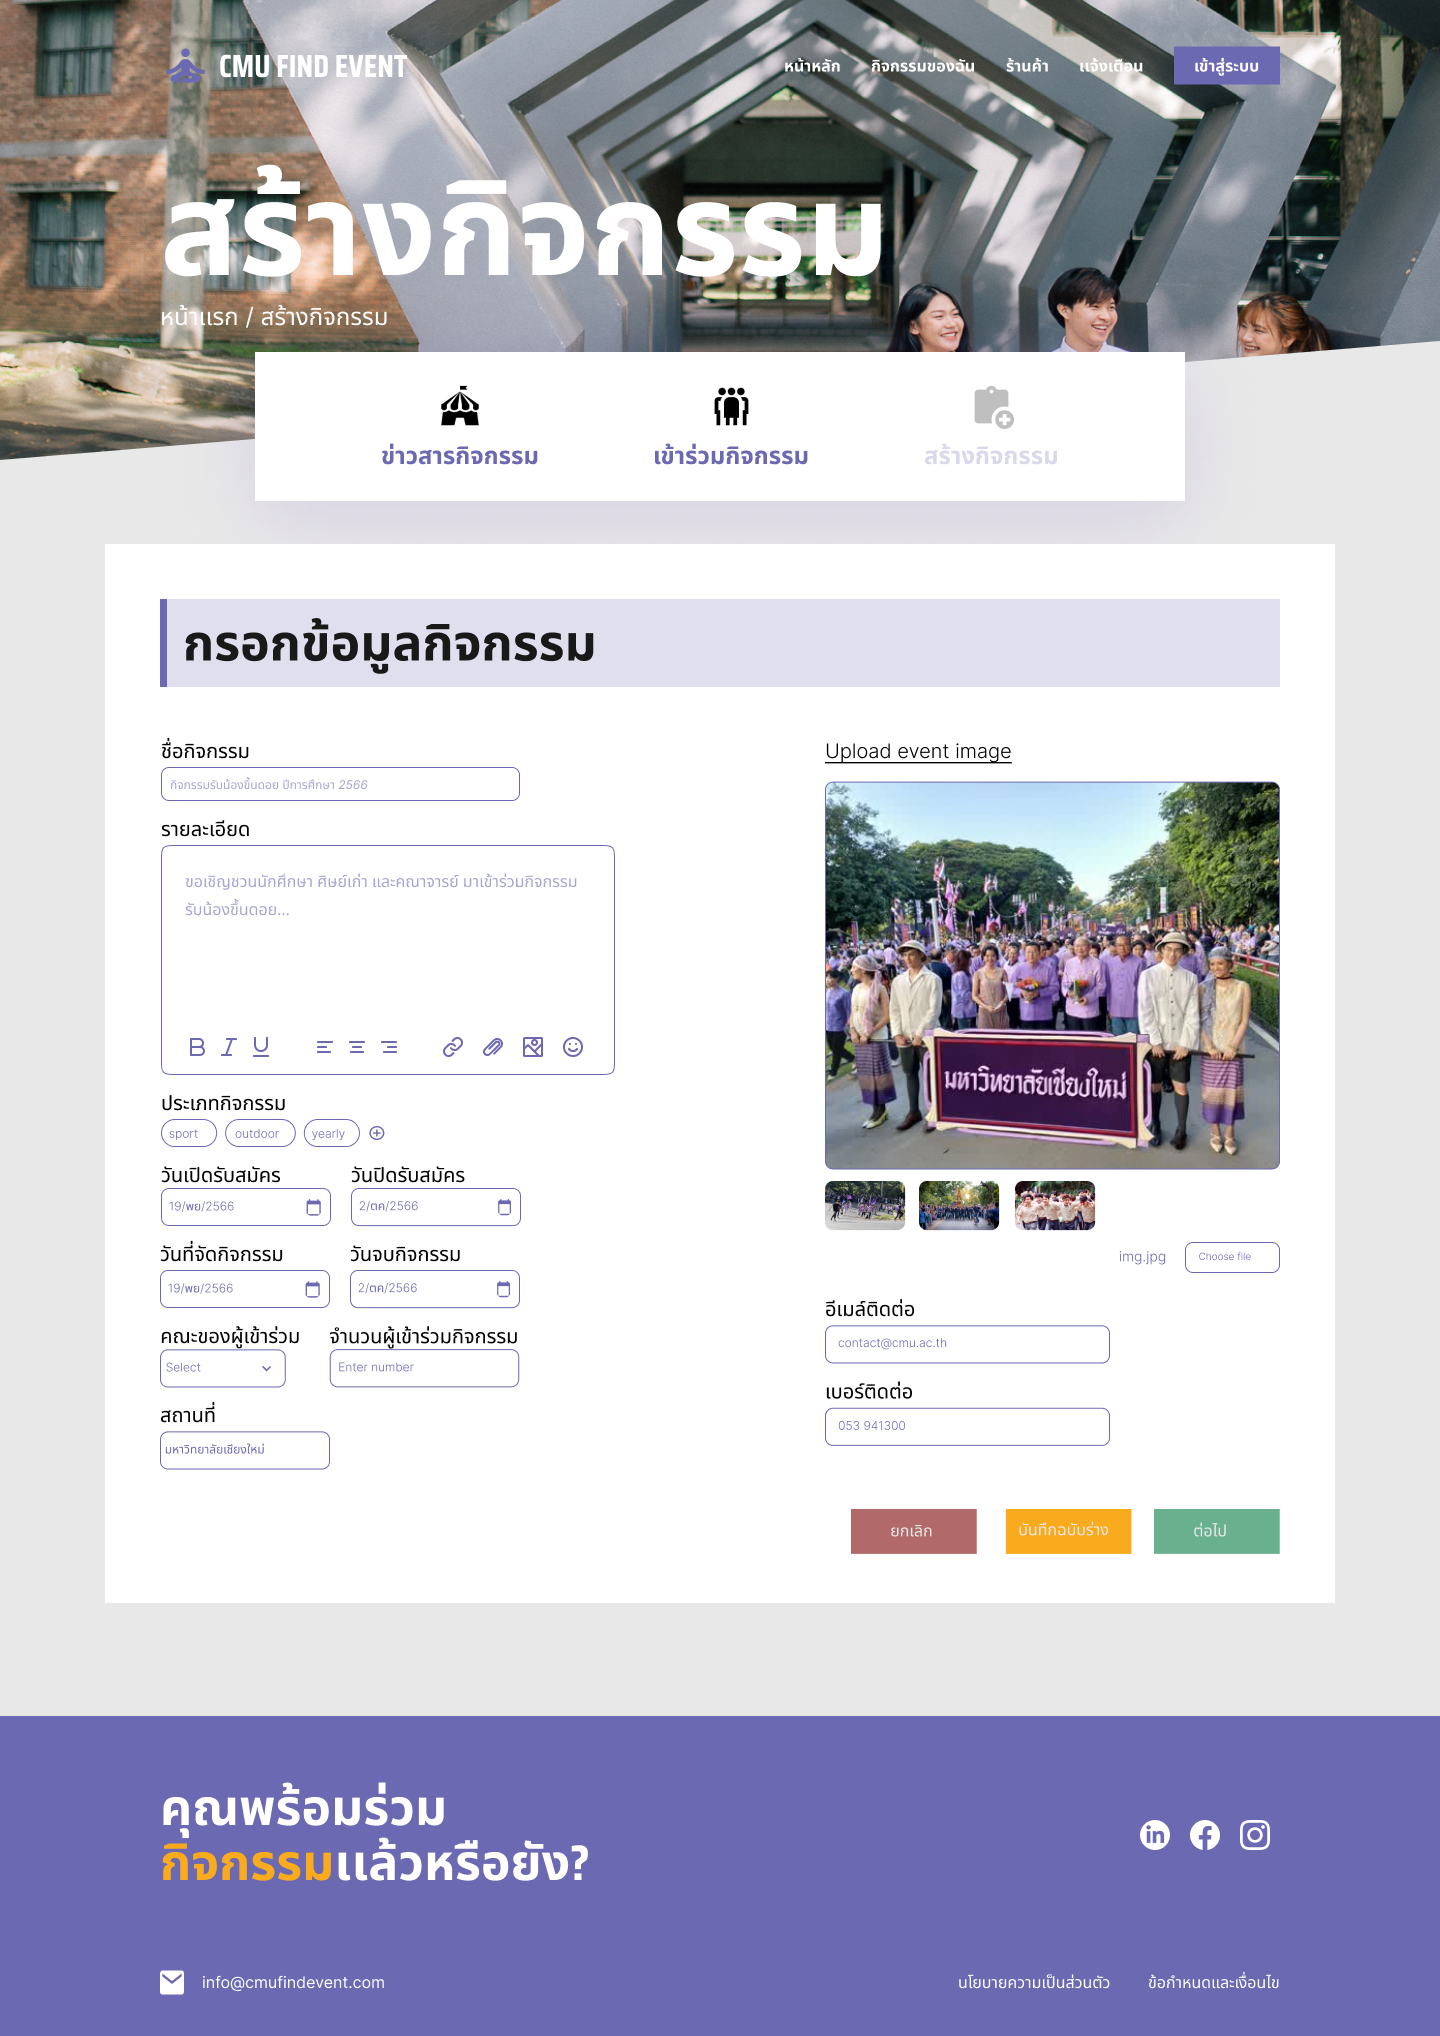
\includegraphics[width=\linewidth]{image/Figma-design/Create-event-info.png}
    \caption{กรอกข้อมูลของกิจกรรม}
  \end{subfigure}
  \hfill
  \begin{subfigure}[b]{0.3\linewidth}
    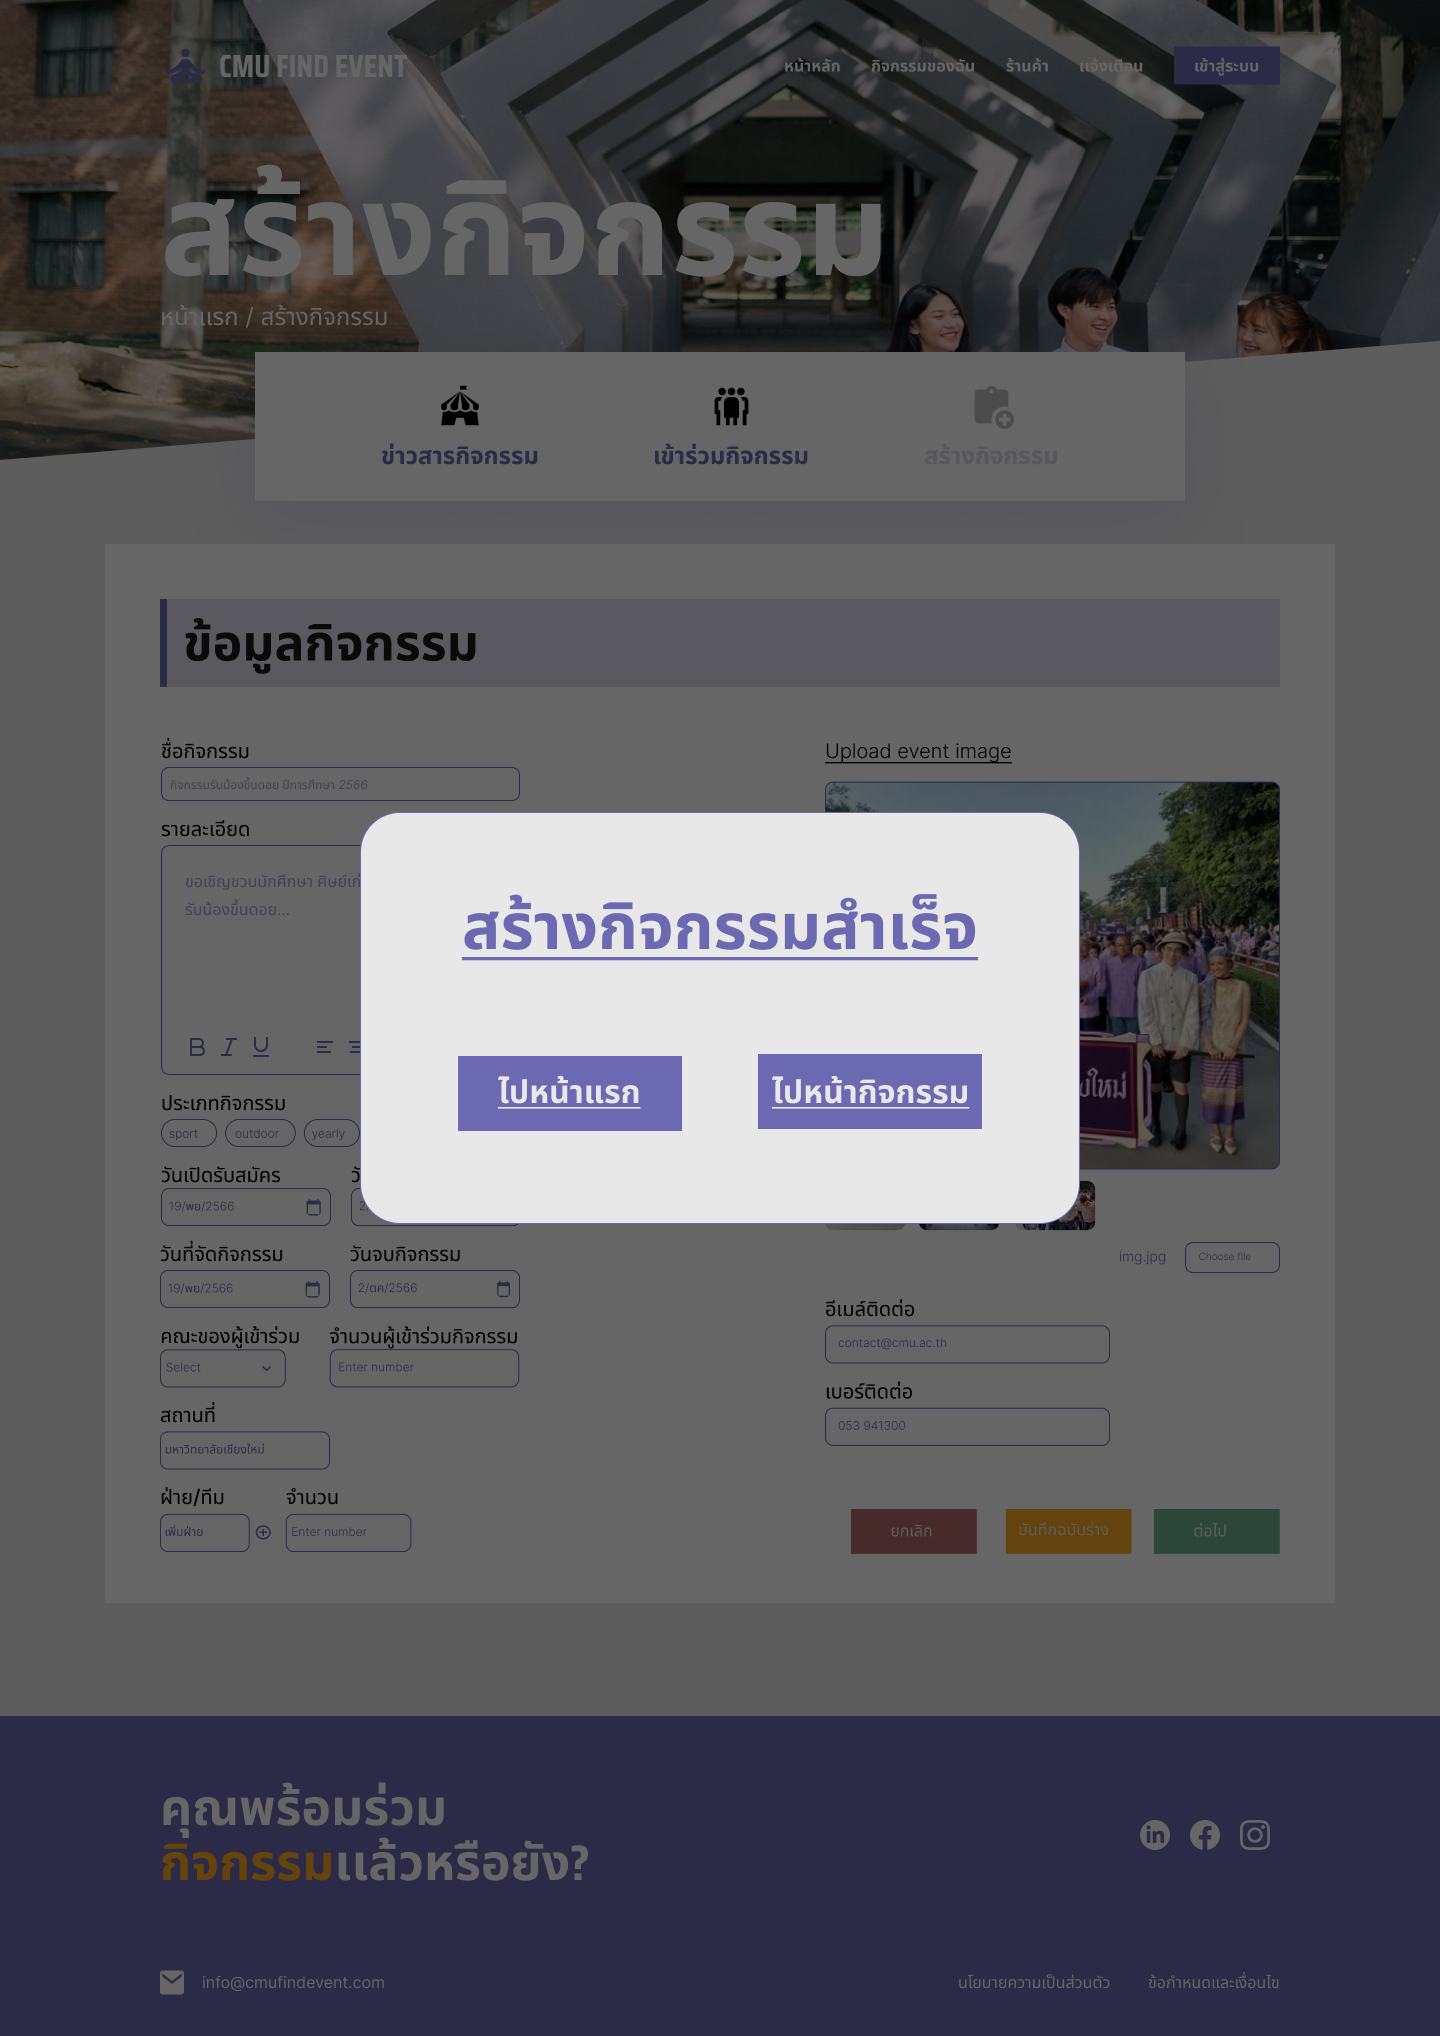
\includegraphics[width=\linewidth]{image/Figma-design/Create-event-info-1.png}
    \caption{แสดงข้อความสร้างสำเร็จ}
  \end{subfigure}
  \caption{หน้าสร้างประกาศกิจกรรม}
  \label{fig:create-event-info}
\end{figure}

\begin{figure}[h]
  \centering
  \begin{subfigure}[b]{0.3\linewidth}
    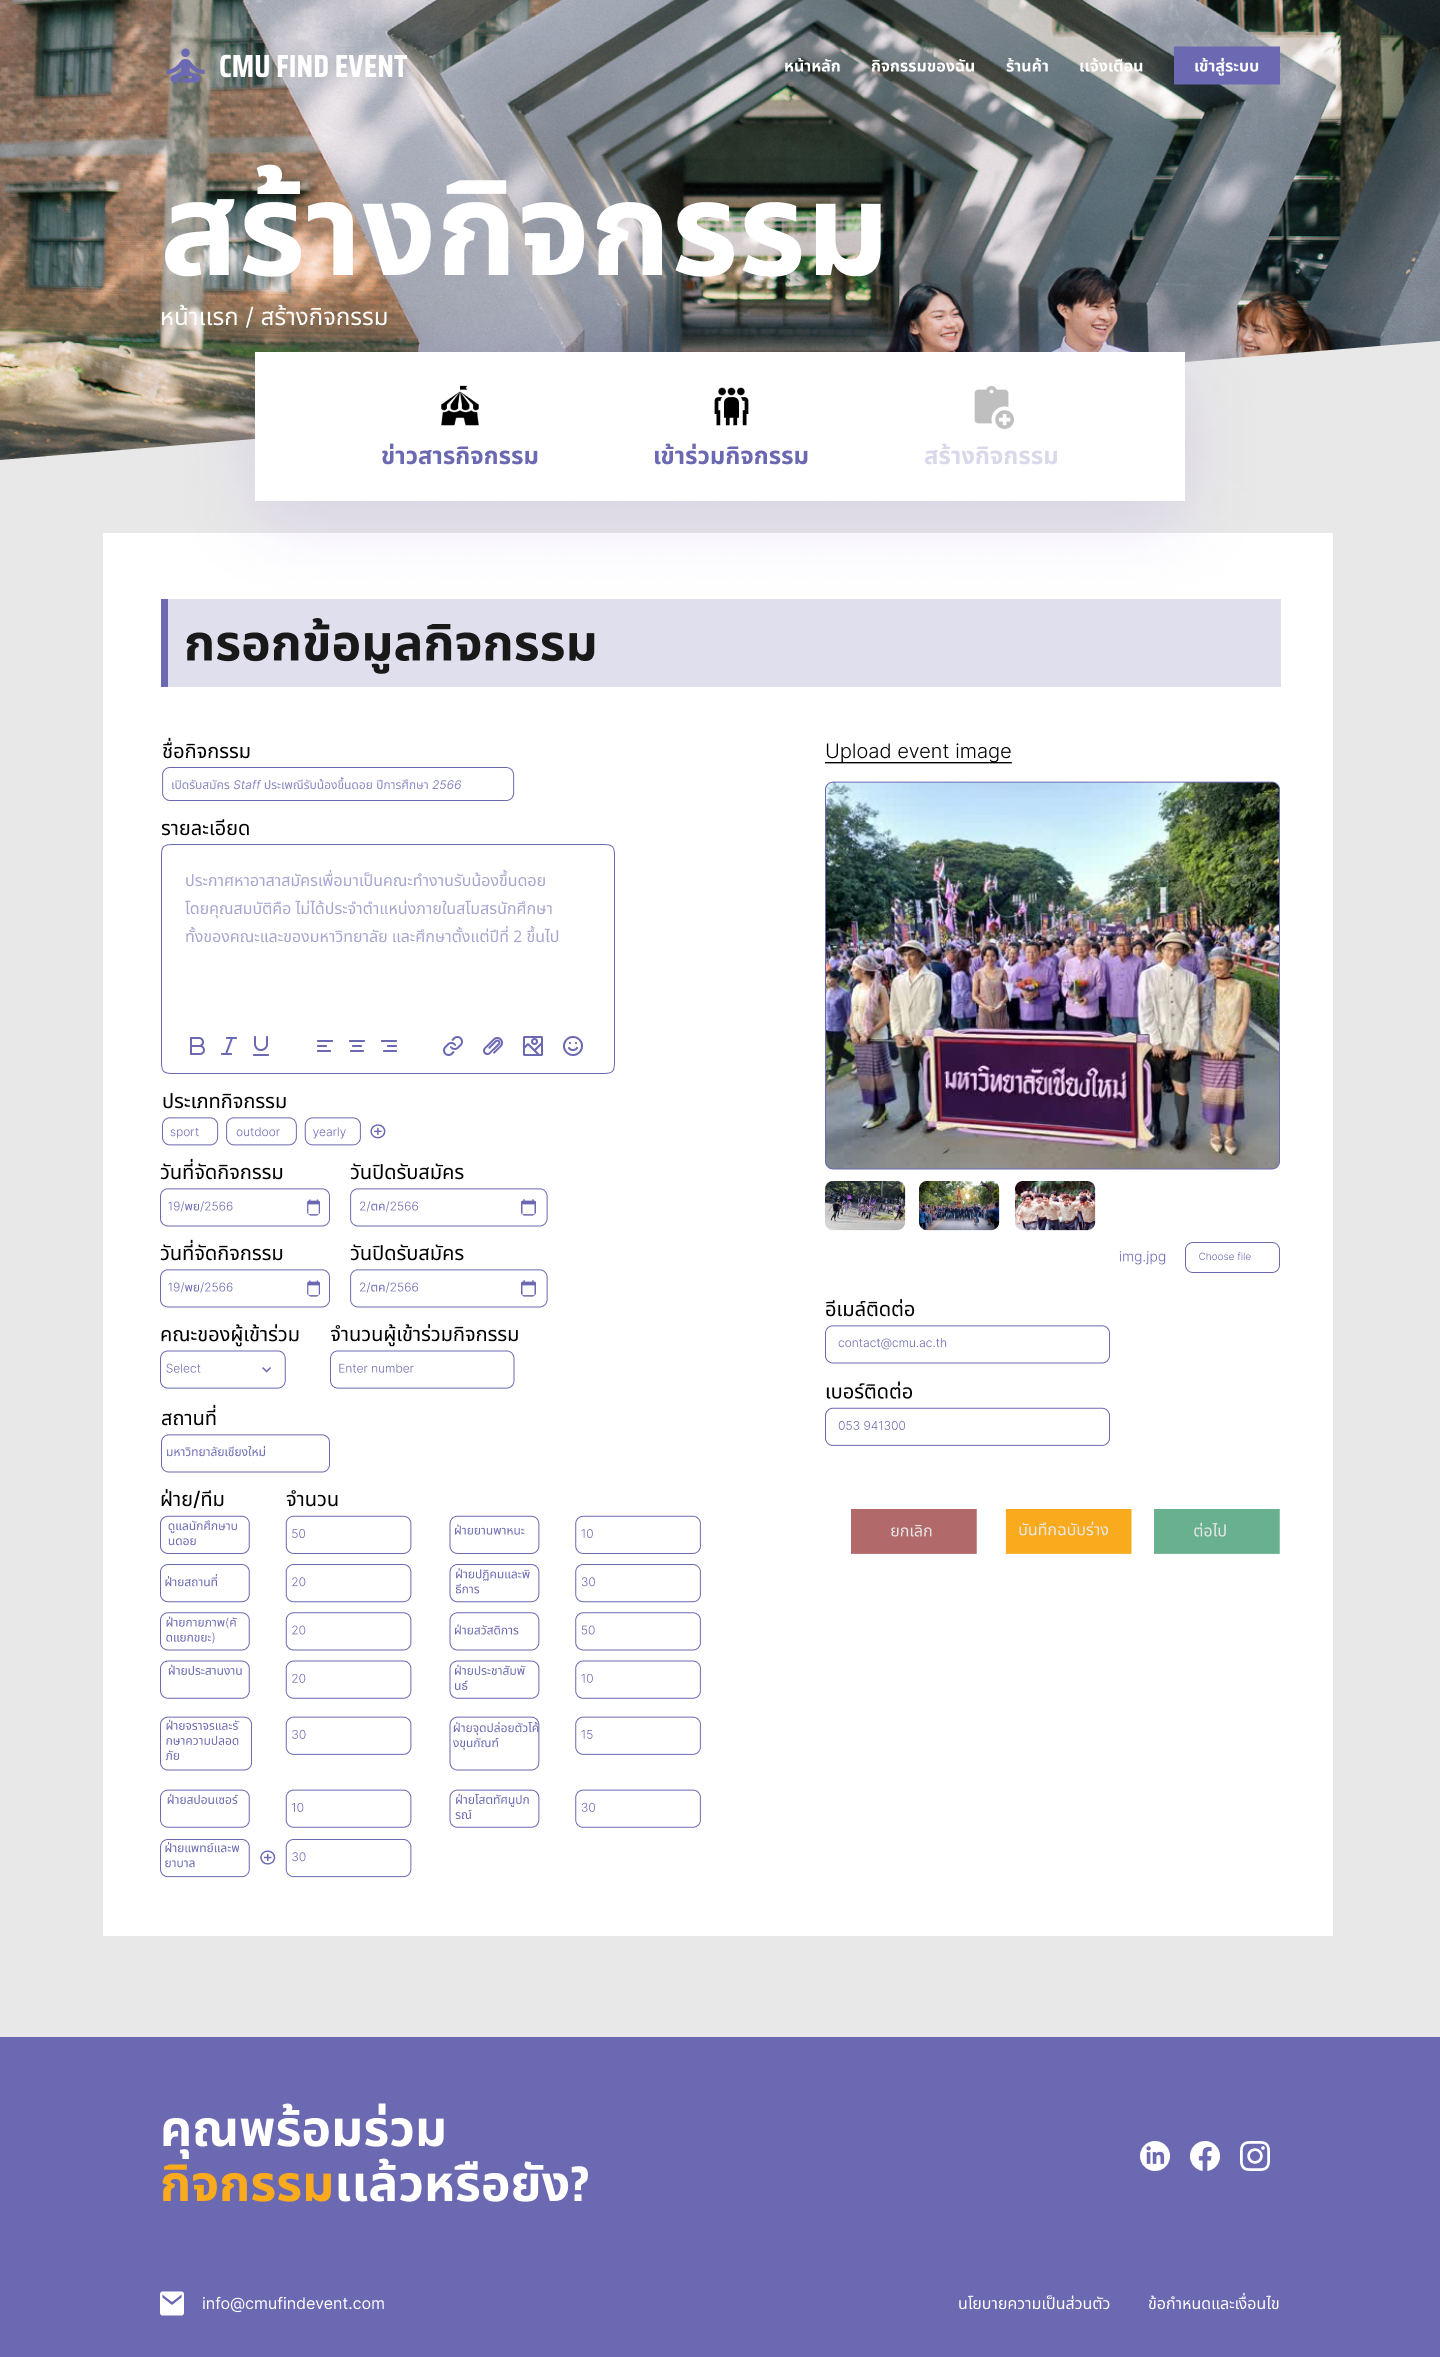
\includegraphics[width=\linewidth]{image/Figma-design/Create-event-join.png}
    \caption{กรอกข้อมูลของกิจกรรม}
  \end{subfigure}
  \hfill
  \begin{subfigure}[b]{0.3\linewidth}
    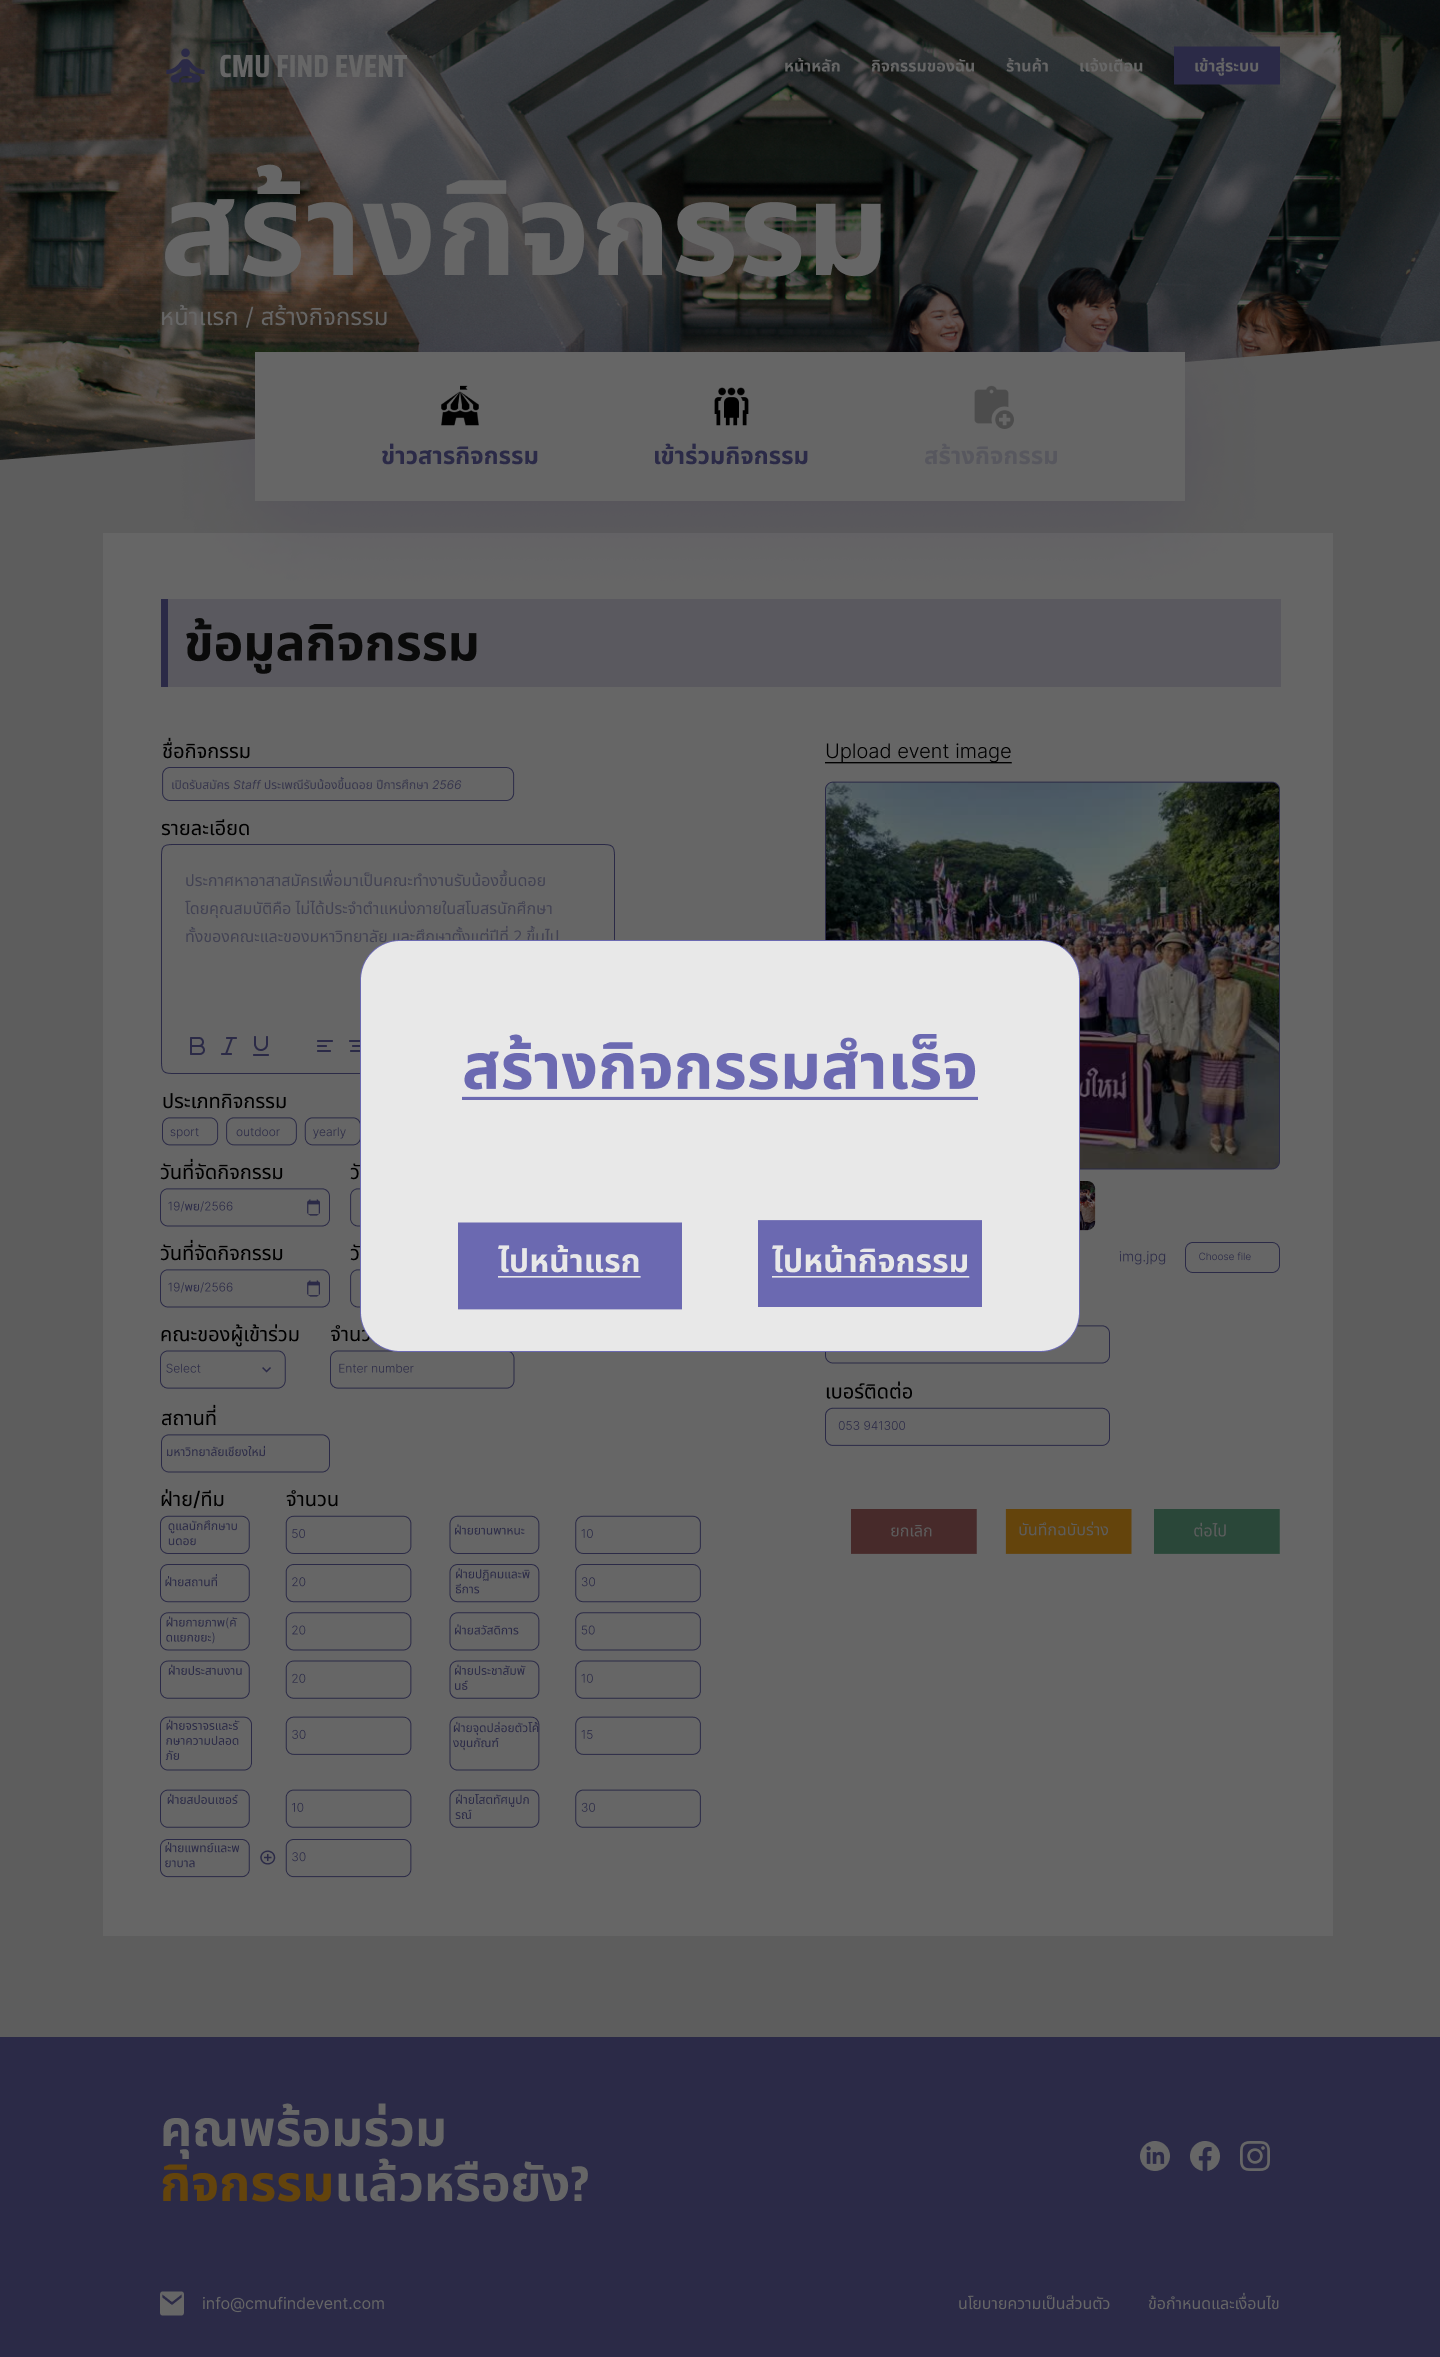
\includegraphics[width=\linewidth]{image/Figma-design/Create-event-join-1.png}
    \caption{แสดงข้อความสร้างสำเร็จ}
  \end{subfigure}
  \caption{หน้าสร้างกิจกรรมแบบรับสมัคร}
  \label{fig:create-event-join}
\end{figure}

\FloatBarrier
\section{โครงสร้างการไหลของข้อมูล}
โครงสร้างการไหลของข้อมูลแบ่งออกเป็น 3 ส่วน ได้แก่ User, System และ Admin
โดยข้อมูลที่userจะส่งไปให้ system ได้แก่ ข้อมูลของผู้ใช้,ข้อมูลการกดสนใจเข้าร่วมกิจกรรม,คำขอเข้าร่วมกิจกรรม,คำขอสร้างกิจกรรม
จากนั้น system จะส่งข้อมูลคำขอสร้างกิจกรรมไปให้ admin ในการอนุมัติ แล้วจึงจะส่งผลการอนุมัติไปพร้อมกับข้อมูลที่จะแสดงผลไปให้ user
ซึ่ง user ที่เป็นผู้สร้างกิจกรรมที่ได้รับคำขอเข้าร่วมกิจกรรม จะสามารถส่งผลการขอเข้าร่วมไปให้ system แล้วส่งต่อให้ user ที่ขอต่อไป ตามดังในรูปภาพที่3.7
\begin{figure}[h]
\begin{center}
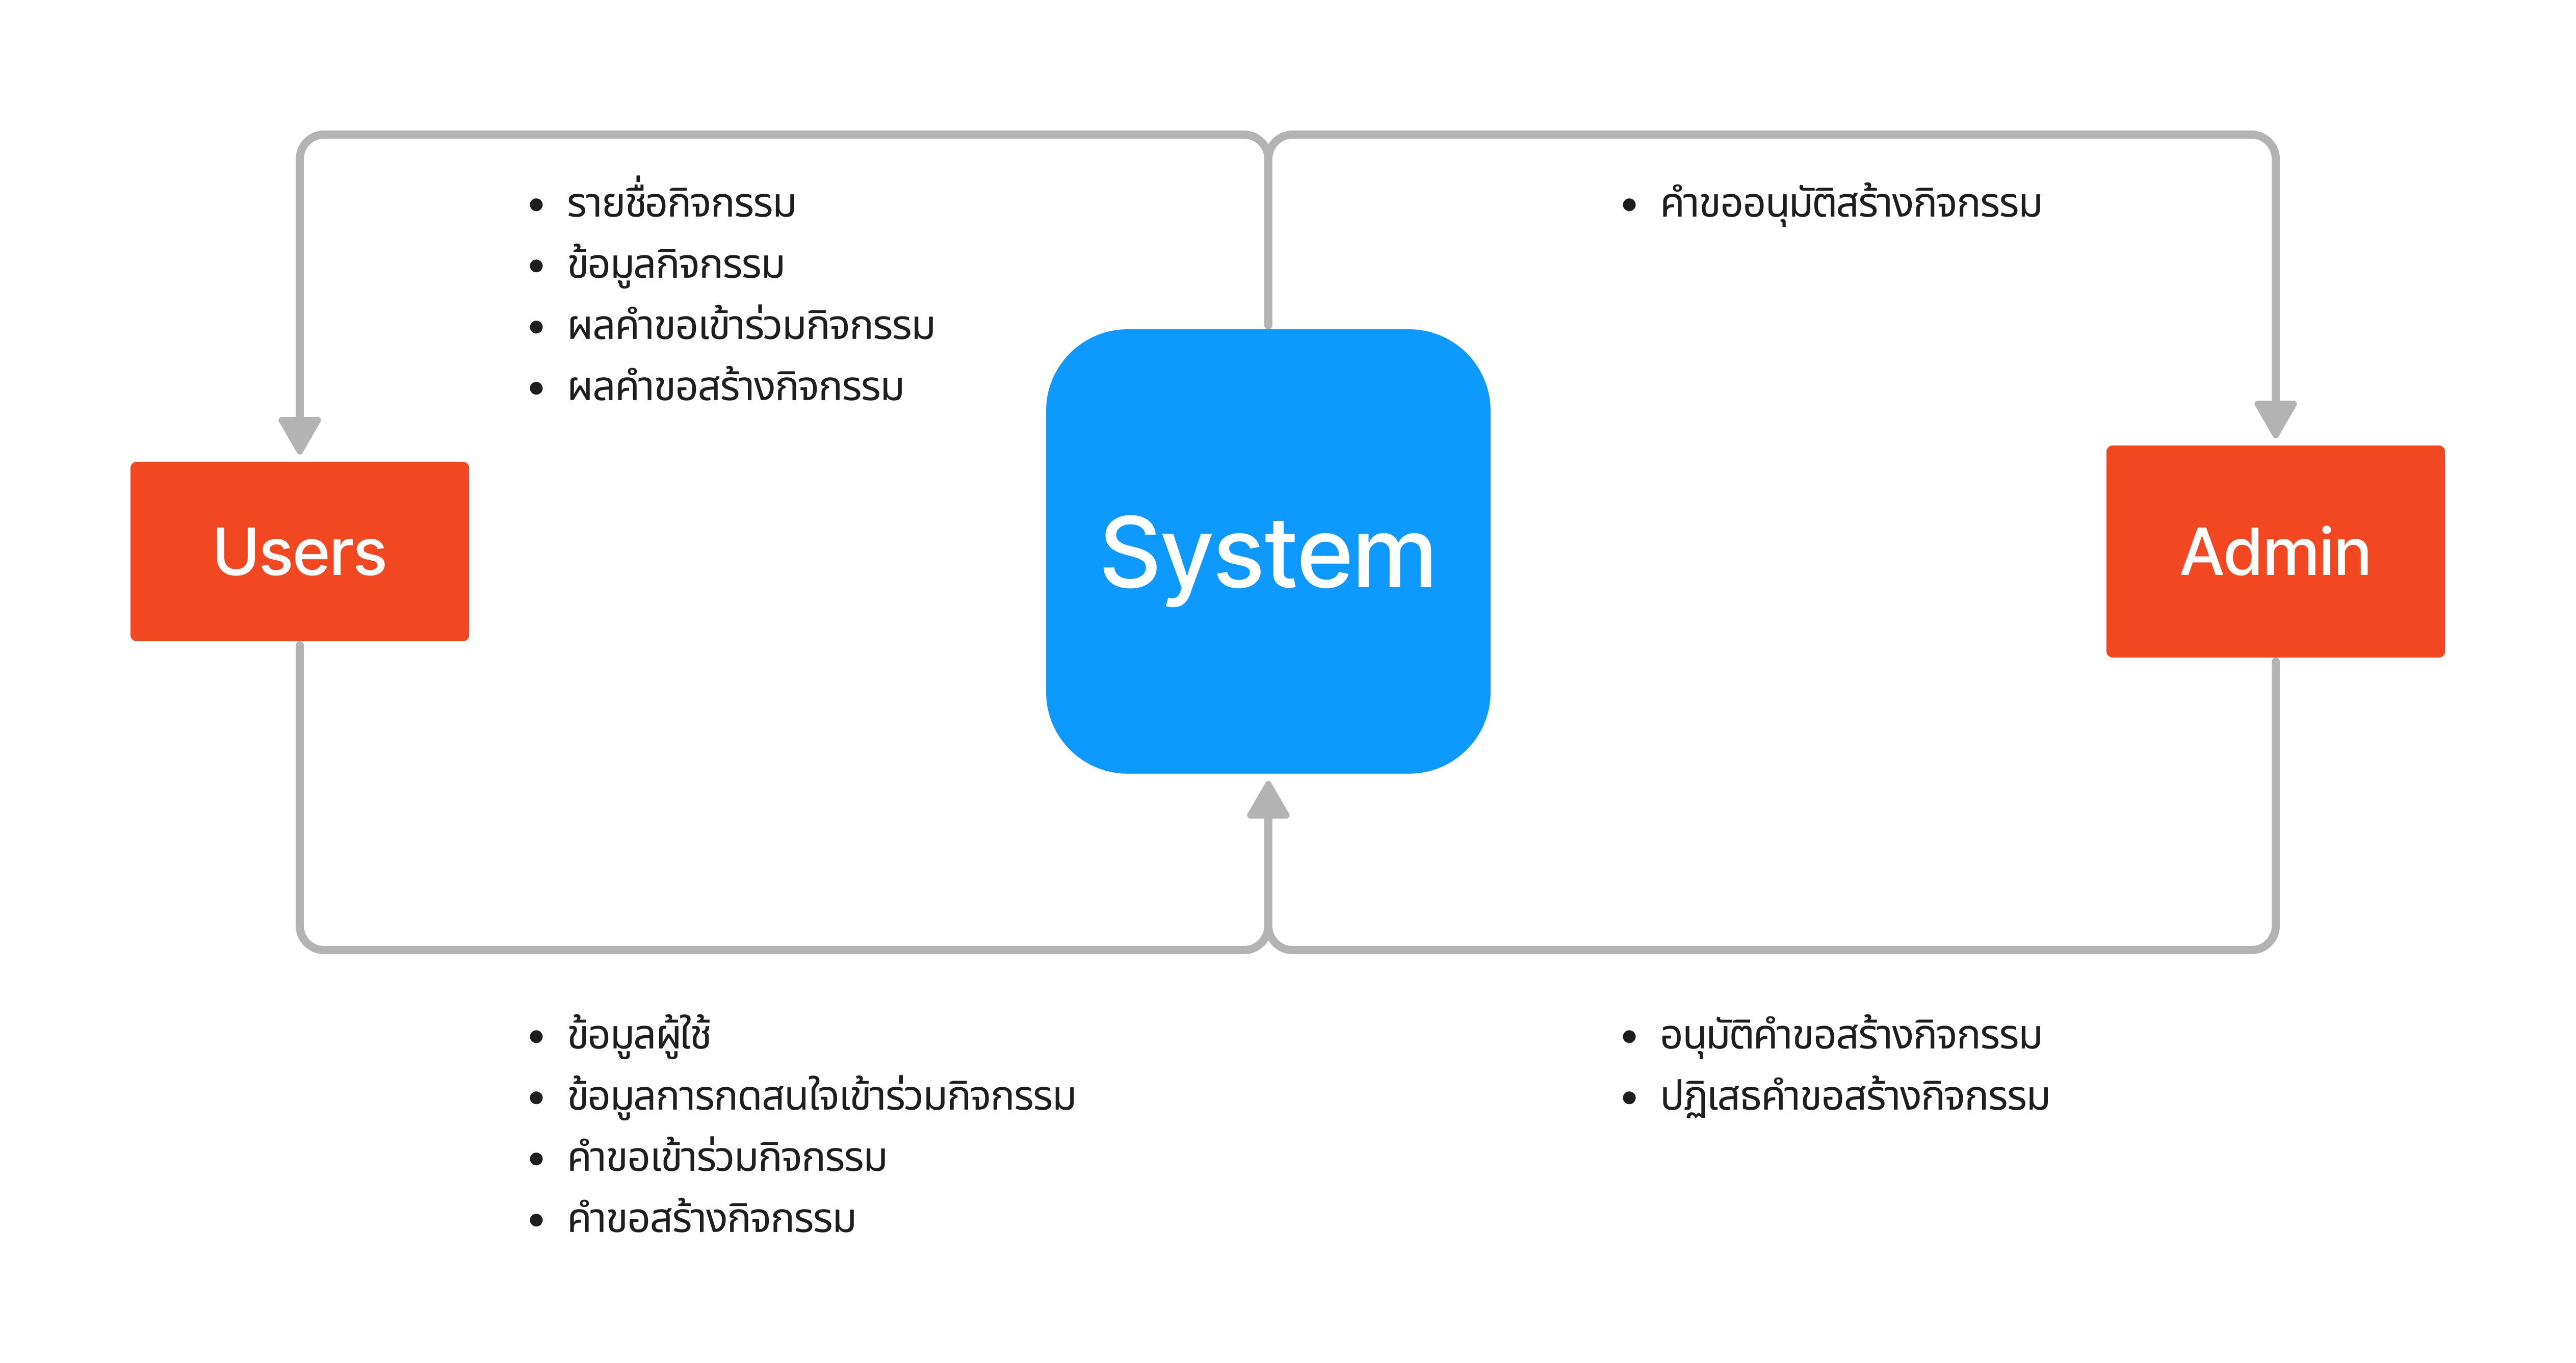
\includegraphics[width=0.9\linewidth]{image/dataflow-diagram.png}
\end{center}
\caption[Poem]{แผนผังการไหลของข้อมูล}
\label{fig:dataflow}
\end{figure}
% \subsection{The Black Kitten}
%   One thing was certain, that the WHITE kitten had had nothing to
% do with it:---it was the black kitten's fault entirely~\cite{aiw}.  For the
% white kitten had been having its face washed by the old cat for
% the last quarter of an hour (and bearing it pretty well,
% considering); so you see that it COULDN'T have had any hand in
% the mischief.

%   The way Dinah washed her children's faces was this:  first she
% held the poor thing down by its ear with one paw, and then with
% the other paw she rubbed its face all over, the wrong way,
% beginning at the nose:  and just now, as I said, she was hard at
% work on the white kitten, which was lying quite still and trying
% to purr---no doubt feeling that it was all meant for its good.

%   But the black kitten had been finished with earlier in the
% afternoon, and so, while Alice was sitting curled up in a corner
% of the great arm-chair, half talking to herself and half asleep,
% the kitten had been having a grand game of romps with the ball of
% worsted Alice had been trying to wind up, and had been rolling it
% up and down till it had all come undone again; and there it was,
% spread over the hearth-rug, all knots and tangles, with the
% kitten running after its own tail in the middle.

% \subsection{The Reproach}

%   `Oh, you wicked little thing!' cried Alice, catching up the
% kitten, and giving it a little kiss to make it understand that it
% was in disgrace.  `Really, Dinah ought to have taught you better
% manners!  You OUGHT, Dinah, you know you ought!' she added,
% looking reproachfully at the old cat, and speaking in as cross a
% voice as she could manage---and then she scrambled back into the
% arm-chair, taking the kitten and the worsted with her, and began
% winding up the ball again.  But she didn't get on very fast, as
% she was talking all the time, sometimes to the kitten, and
% sometimes to herself.  Kitty sat very demurely on her knee,
% pretending to watch the progress of the winding, and now and then
% putting out one paw and gently touching the ball, as if it would
% be glad to help, if it might.

%   `Do you know what to-morrow is, Kitty?' Alice began.  `You'd
% have guessed if you'd been up in the window with me---only Dinah
% was making you tidy, so you couldn't.  I was watching the boys
% getting in stick for the bonfire---and it wants plenty of
% sticks, Kitty!  Only it got so cold, and it snowed so, they had
% to leave off.  Never mind, Kitty, we'll go and see the bonfire
% to-morrow.'  Here Alice wound two or three turns of the worsted
% round the kitten's neck, just to see how it would look:  this led
% to a scramble, in which the ball rolled down upon the floor, and
% yards and yards of it got unwound again.

%   `Do you know, I was so angry, Kitty,' Alice went on as soon as
% they were comfortably settled again, `when I saw all the mischief
% you had been doing, I was very nearly opening the window, and
% putting you out into the snow!  And you'd have deserved it, you
% little mischievous darling!  What have you got to say for
% yourself?  Now don't interrupt me!' she went on, holding up one
% finger.  `I'm going to tell you all your faults.  Number one:
% you squeaked twice while Dinah was washing your face this
% morning.  Now you can't deny it, Kitty:  I heard you!  What that
% you say?' (pretending that the kitten was speaking.)  `Her paw
% went into your eye?  Well, that's YOUR fault, for keeping your
% eyes open---if you'd shut them tight up, it wouldn't have
% happened.  Now don't make any more excuses, but listen!  Number
% two:  you pulled Snowdrop away by the tail just as I had put down
% the saucer of milk before her!  What, you were thirsty, were you?

\ifproject
\chapter{\ifproject%
\ifenglish Experimentation and Results\else การทดลองและผลลัพธ์\fi
\else%
\ifenglish System Evaluation\else การประเมินระบบ\fi
\fi}

\hspace{4ex} 
ในบทนี้จะกล่าวถึงผลการทดสอบการทำงานของเว็บแอปพลิเคชัน โดยจะแบ่งเป็นหมวดฟีเจอร์หลัก และหมวดฟีเจอร์เสริม โดยจะทำการทดสอบผ่านหน้าเว็บแอปพลิเคชัน

\section{ผลการทดสอบการทำงานฟีเจอร์หลัก}

\section{ผลการทดสอบการทำงานฟีเจอร์เสริม}
\chapter{\ifenglish Conclusions and Discussions\else บทสรุปและข้อเสนอแนะ\fi}

\section{\ifenglish Conclusions\else สรุปผล\fi}

\hspace{4ex} 
จากการพัฒนาโครงงาน Project Matching Management Platform ระบบที่ได้ สามารถทำงานได้ตามวัตถุประสงค์ของโครงงานซึ่งก็คือสามารถพัฒนาเว็บแอปพลิเคชันที่สามารถรองรับการประกาศกิจกรรมและเข้าร่วมกิจกรรมได้อย่างถูกต้อง อีกทั้งสามารถพัฒนาระบบที่สามารถนำข้อมูลของผู้ใช้มาใช้ในการแนะนำกิจกรรมให้กับผู้ใช้ได้

\section{\ifenglish Challenges\else ปัญหาที่พบและแนวทางการแก้ไข\fi}

ในการทำโครงงานนี้ พบว่าเกิดปัญหาหลักๆ ดังนี้
\begin{enumerate}
    \item การพูดคุยระหว่างผู้พัฒนามีจำนวนน้อยเกินไปทำให้งานดำเนินไปได้ด้วยความล่าช้า และทำให้เกิดปัญหาในการดำเนินงาน
    \item ไม่สามารถหาข้อมูลสถิติการเข้าร่วมกิจกรรมต่างๆของนักศึกษาแบ่งตามแท็กกิจกรรมได้ ทำให้ระบบแนะนำกิจกรรมที่ได้มีประสิทธิภาพไม่เป็นอย่างที่ออกแบบไว้
    \item คิดออกแบบโครงงานได้ไม่ดีเพียงพอ ทำให้ตอนพัฒนาจริงต้องปรับเปลี่ยนอะไรต่างๆจากที่ออกแบบไว้มากกว่าที่ควร
    \item วางแผนเวลาการดำเนินงานได้ไม่ดีพอ และ ใช้เวลาในการคิดออกแบบระบบต่างๆมากเกินไป แล้วไม่ได้ลงมือปฏิบัติจริงซักที ทำให้เวลาในการพัฒนาไม่เพียงพอ
\end{enumerate}

\section{\ifenglish%
Suggestions and further improvements
\else%
ข้อเสนอแนะและแนวทางการพัฒนาต่อ
\fi
}

ข้อเสนอแนะเพื่อพัฒนาโครงงานนี้ต่อไป มีดังนี้

\begin{enumerate}
    \item พัฒนาระบบแนะนำจากการนำข้อมูลของแท็กของผู้ใช้ไปทำการเสิร์ช เป็นการนำข้อมูลต่างๆของผู้ใช้ไปทำการประมวลผลหาแนวโน้มร่วมกับผู้ใช้อื่นๆด้วย
    \item จัดการเคลียร์โค้ดใหม่ให้มีประสิทธิภาพมากยิ่งขึ้น 
    \item พัฒนาระบบให้สามารถใช้กับ CMU Account ได้
    \item เพิ่มระบบการจัดการสมาชิกในกิจกรรม
    \item เพิ่มระบบรีวิวกิจกรรม
    \item เพิ่มการทำงานฝั่ง Admin
    \item เพิ่มระบบสรุปผลการเข้าร่วมกิจกรรมของผู้ใช้
    \item นำเว็บแอปพลิเคชันไป deploy บน Cloud
\end{enumerate}

\fi

\bibliography{sampleReport}

\ifproject
\normalspacing
\appendix
% \chapter{The first appendix}

% Text for the first appendix goes here.

% \section{Appendix section}

% Text for a section in the first appendix goes here.

% test ทดสอบฟอนต์ serif ภาษาไทย

% \textsf{test ทดสอบฟอนต์ sans serif ภาษาไทย}

% \verb+test ทดสอบฟอนต์ teletype ภาษาไทย+

% \texttt{test ทดสอบฟอนต์ teletype ภาษาไทย}

% \textbf{ตัวหนา serif ภาษาไทย \textsf{sans serif ภาษาไทย} \texttt{teletype ภาษาไทย}}

% \textit{ตัวเอียง serif ภาษาไทย \textsf{sans serif ภาษาไทย} \texttt{teletype ภาษาไทย}}

% \textbf{\textit{ตัวหนาเอียง serif ภาษาไทย \textsf{sans serif ภาษาไทย} \texttt{teletype ภาษาไทย}}}

% \url{https://www.example.com/test_ทดสอบ_url}

\chapter{\ifenglish Manual\else คู่มือการใช้งานระบบ\fi}

สามารถดูรายละเอียดต่างๆของโครงงานได้ที่
\href{https://github.com/Thidtanai/Thidtanai-PMMP-261492.git}{Github}.



%% Display glossary (optional) -- need glossary option.
\ifglossary\glossarypage\fi

%% Display index (optional) -- need idx option.
\ifindex\indexpage\fi

\begin{biosketch}
\begin{center}
  \includegraphics[width=1.5in]{mugshot.jpg}
\end{center}
Your biosketch goes here. Make sure it sits inside
the \texttt{biosketch} environment.
\end{biosketch}
\fi % \ifproject
\end{document}
